\documentclass{beamer}
\usepackage{transparent}
\usepackage[beamer]{shortcut}


\usepackage{animate}
\usepackage{bibentry}
\usepackage{subcaption}
\usepackage{appendixnumberbeamer}

\graphicspath{{../thesis/figures/},{./images/}}
\def\TikzLocation{./tikz/}
\def\tkzscl{1}

\def\twocols{}
%\def\bimplies{}
%\def\partintro{}


\definecolor{primary}{RGB}{191,213,219}
\definecolor{secondary}{RGB}{144,106,66}
\setbeamercolor{block title}{fg=darkred}
\newcommand{\btitle}[1]{{\usebeamerfont{block title}\usebeamercolor[fg]{block title} #1}}

\AtBeginSection[]
{
}


\makeatletter
\def\beamer@newblock{%
  \usebeamercolor[fg]{bibliography entry author}%
  \usebeamerfont{bibliography entry author}%
  \usebeamertemplate{bibliography entry author}%
  \def\newblock{%
    \usebeamercolor[fg]{bibliography entry title}%
    \usebeamerfont{bibliography entry title}%
    \usebeamertemplate{bibliography entry title}%
    \def\newblock{%
      \usebeamercolor[fg]{bibliography entry location}%
      \usebeamerfont{bibliography entry location}%
      \usebeamertemplate{bibliography entry location}%
      \def\newblock{%
        \usebeamercolor[fg]{bibliography entry note}%
        \usebeamerfont{bibliography entry note}%
        \usebeamertemplate{bibliography entry note}}}}%
  \leavevmode\setbox\beamer@tempbox=\hbox{}\ht\beamer@tempbox=0em\box\beamer@tempbox}
  \setbeamertemplate{bibliography entry title}{}{}

\makeatother

\usepackage[square, authoryear]{natbib}


%-----------------------------------------------------------------------------
%	CUSTOM COMANDS
%-----------------------------------------------------------------------------

\def\keypoint#1{\hspace{0pt plus 1 filll}\textcolor{gray}{#1}}
\def\mycite#1{\keypoint{\small\citep{#1}}}
\def\citeconf#1#2{
    {\textcolor{gray}[}%
        {\color{linkcolor}\citealt{#1}, #2}%
    {\textcolor{gray}]}}
\def\citeconfright#1#2{\hspace{0pt plus 1 filll}{\small\citeconf{#1}{#2}}}
\def\biblio{
	\nobibliography{../../library}
	\def\biblio{}
}




%\usepackage{lxfonts}

\institute{-- INRIA -- Université Paris Saclay}
\author{Thomas Moreau}
\title{Using the Dictionary Structure\\for efficient\\Convolutional Dictionary Learning}


\setbeamertemplate{title page}[frame]


\begin{document}

\begin{frame}[plain]
\titlepage
\biblio{}
\end{frame}

\def\biblio{}


\subfile{motiv}


%========================================================================
\section{Adaptive Sparse Coding}
\label{sec:lista}
%========================================================================
\parttitleframe{Moreau2017}

\subfile{lista}


%========================================================================
\section{Scaling up Convolutional Sparse Coding with coordinate descent and distributed optimization}
\label{sec:lgcd}
%========================================================================

\parttitleframe{Moreau2018, Moreau2019}
\subfile{dicod}


%========================================================================
\section{Rank-1 Constrained Convolutional Dictionary Learning}
\label{sec:multicsc}
%========================================================================

\parttitleframe{Dupre2018}
\subfile{multicsc}


%===========================================================================
\section{Conclusion}
%===========================================================================

\begin{frame}{Conclusion}
    \textbf{Convolutional Dictionary Learning}
    \begin{itemize}\itemsep.5em
        \item Flexible pattern extraction technique,
        \item Computationally tractable for more and more problems,
        \item Some application are already beginning to emerge.
    \end{itemize}
    \vskip2em
    \textbf{Challenges}
    \begin{itemize}\itemsep.5em
        \item Theoretical challenges remains (convergence, recoverability),
        \item The evaluation (and thus the parameter choices) is still not clear,
        \item Can give some insight for deep learning models?
    \end{itemize}
\end{frame}


\begin{frame}{}
\vskip2em
{\centering
    \usebeamercolor[fg]{title}
    \usebeamerfont{title}
    \Huge \bf Thanks!\\[2em]}

Code available online:\\[1em]


\includegraphics[height=.8em]{github}~\textbf{LISTA} : github.com/tommoral/AdaptiveOptim\\[1em]

\includegraphics[height=.8em]{github}~\textbf{DICOD} (\& DiCoDiLe soon) : github.com/tommoral/dicod\\[1em]

\includegraphics[height=.8em]{github}~\textbf{alphacsc} :  alphacsc.github.io\\[2em]

Slides are on my web page:\\[1em]
\hskip5em\includegraphics[height=.8em]{website} tommoral.github.io
\hskip4em 
\includegraphics[height=.8em]{twitter} @tomamoral


\end{frame}
%===========================================================================
% AUXILIARY SLIDES
%===========================================================================



%===========================================================================
\appendix
\section{Auxiliary Slides}
%===========================================================================


%===========================================================================
\subsection{Physiological Signals}
%===========================================================================

\begin{frame}{Signals from human walking}
\centering
\vskip1em
\begin{tabular}{m{8em} m{20em}}
    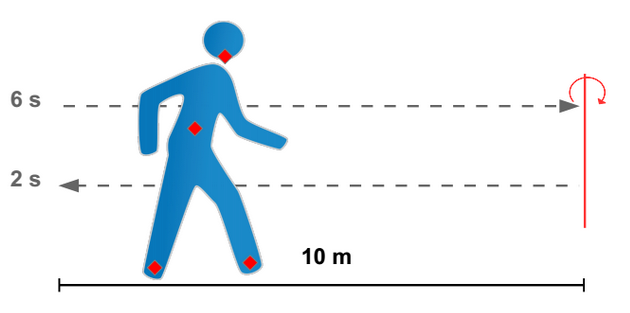
\includegraphics[width=.3\textwidth]{exo_marche}
    \raisebox{-.5\height}{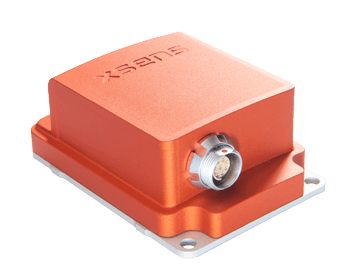
\includegraphics[width=.15\textwidth]{xsens}} $\substack{\text{Inertial}\\\text{captor}}$ &
    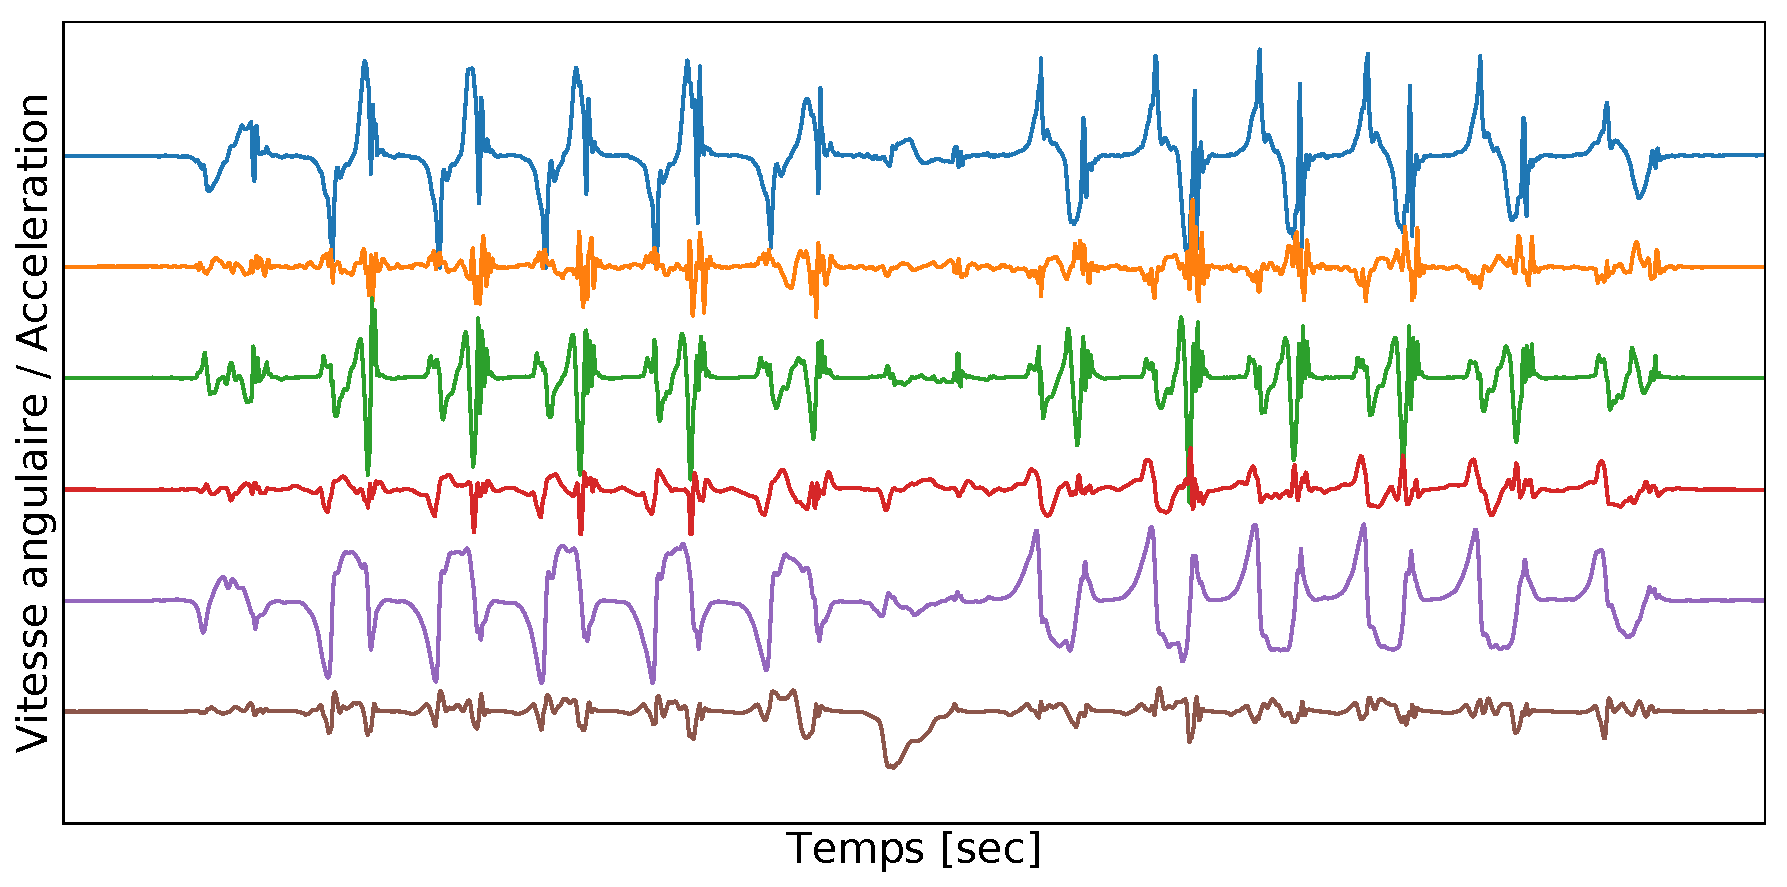
\includegraphics[width=.6\textwidth]{accelero}
\end{tabular}
\vskip1em
\begin{itemize}
    \item Shift invariant patterns linked to steps,
    \item Manual segmentation of the signal is expensive.
\end{itemize}
\strongpoint{Can we do better with data-driven approach?}

\end{frame}



\begin{frame}{Experiment}
		Create a dictionary with 25 Gaussian patterns ($W=90$)
		\[
			\pmb D^{(0)}_k \sim \mathcal N(0, I_{90})
		\]
		\vskip1em
		Use the Convolutional Dictionary Learning with\\
		DICOD to learn a dictionary $\pmb D$ on a set of $50$\\
		recording of healthy subjects walking.
		\vskip2em
		\btitle{Challenges}
		\vskip.5em
		\begin{itemize}\itemsep.5em
			\item Alignment of the patterns,
			\item Detect steps of different amplitude,
			\item Handle multivariate signals.
		\end{itemize}

\end{frame}
\begin{frame}{Experiment}
		\centering
		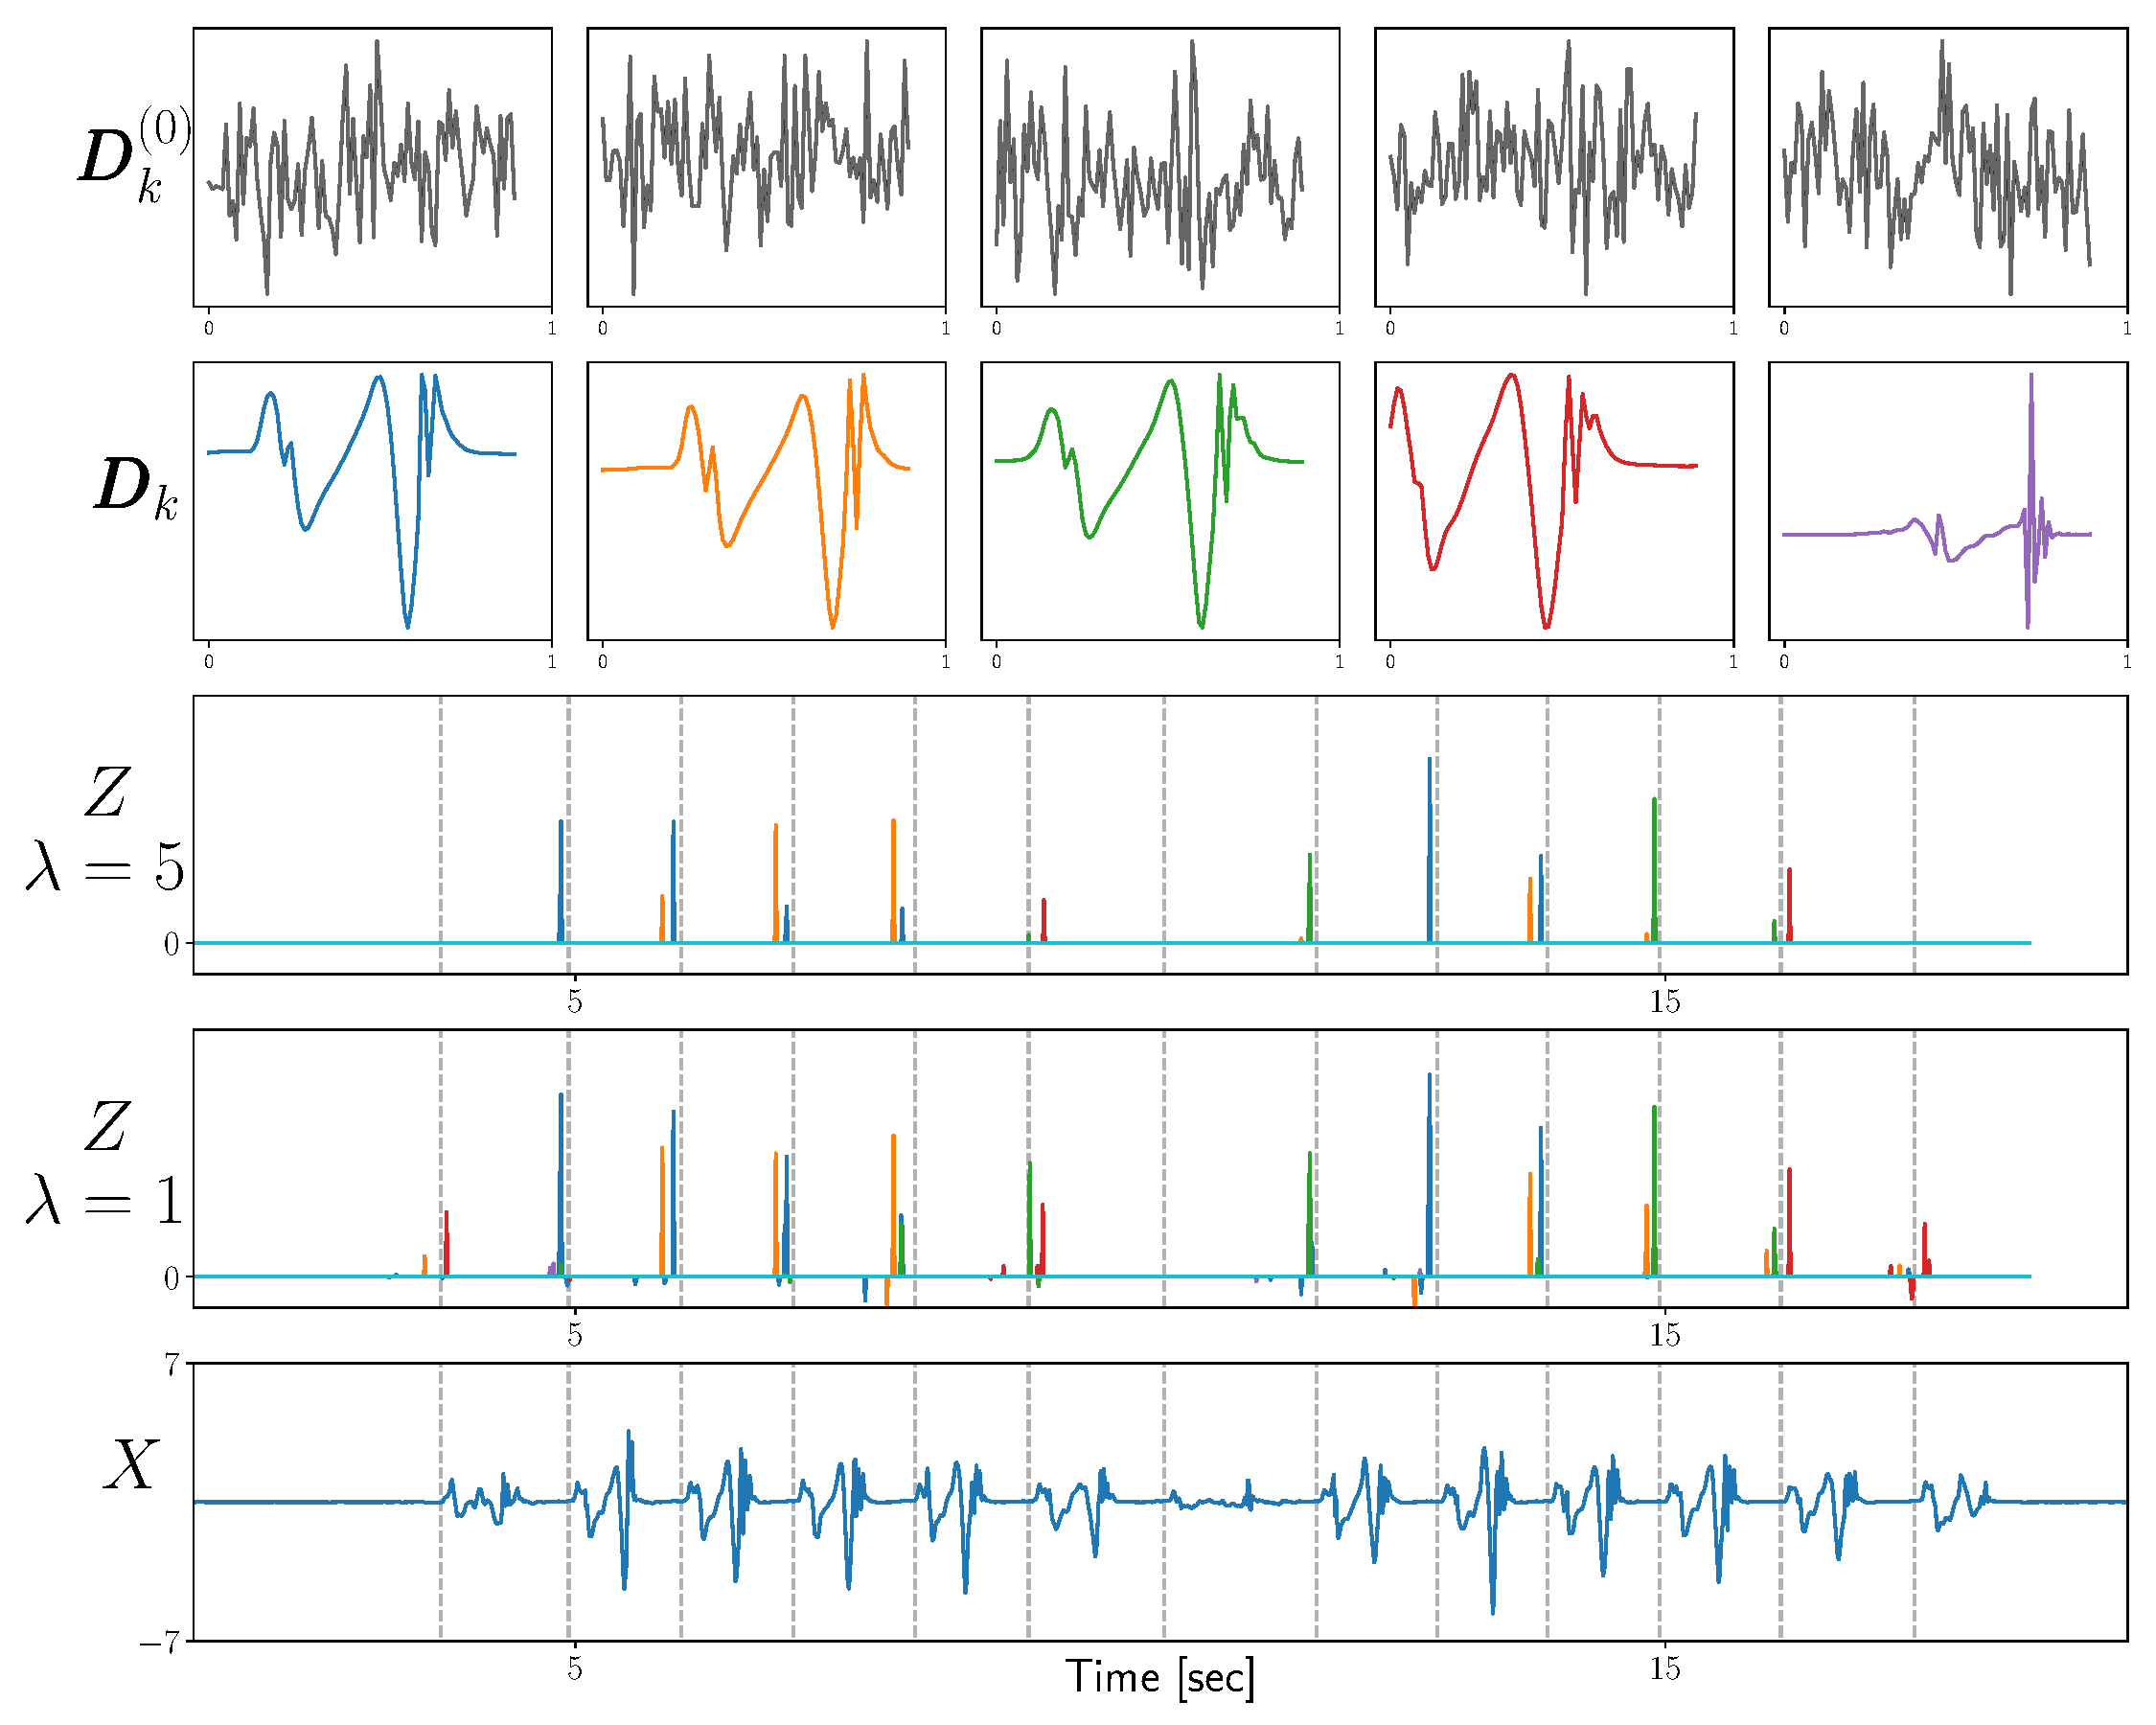
\includegraphics[width=.8\textwidth]{csc_random_defense}

\end{frame}


\begin{frame}
	\centering
	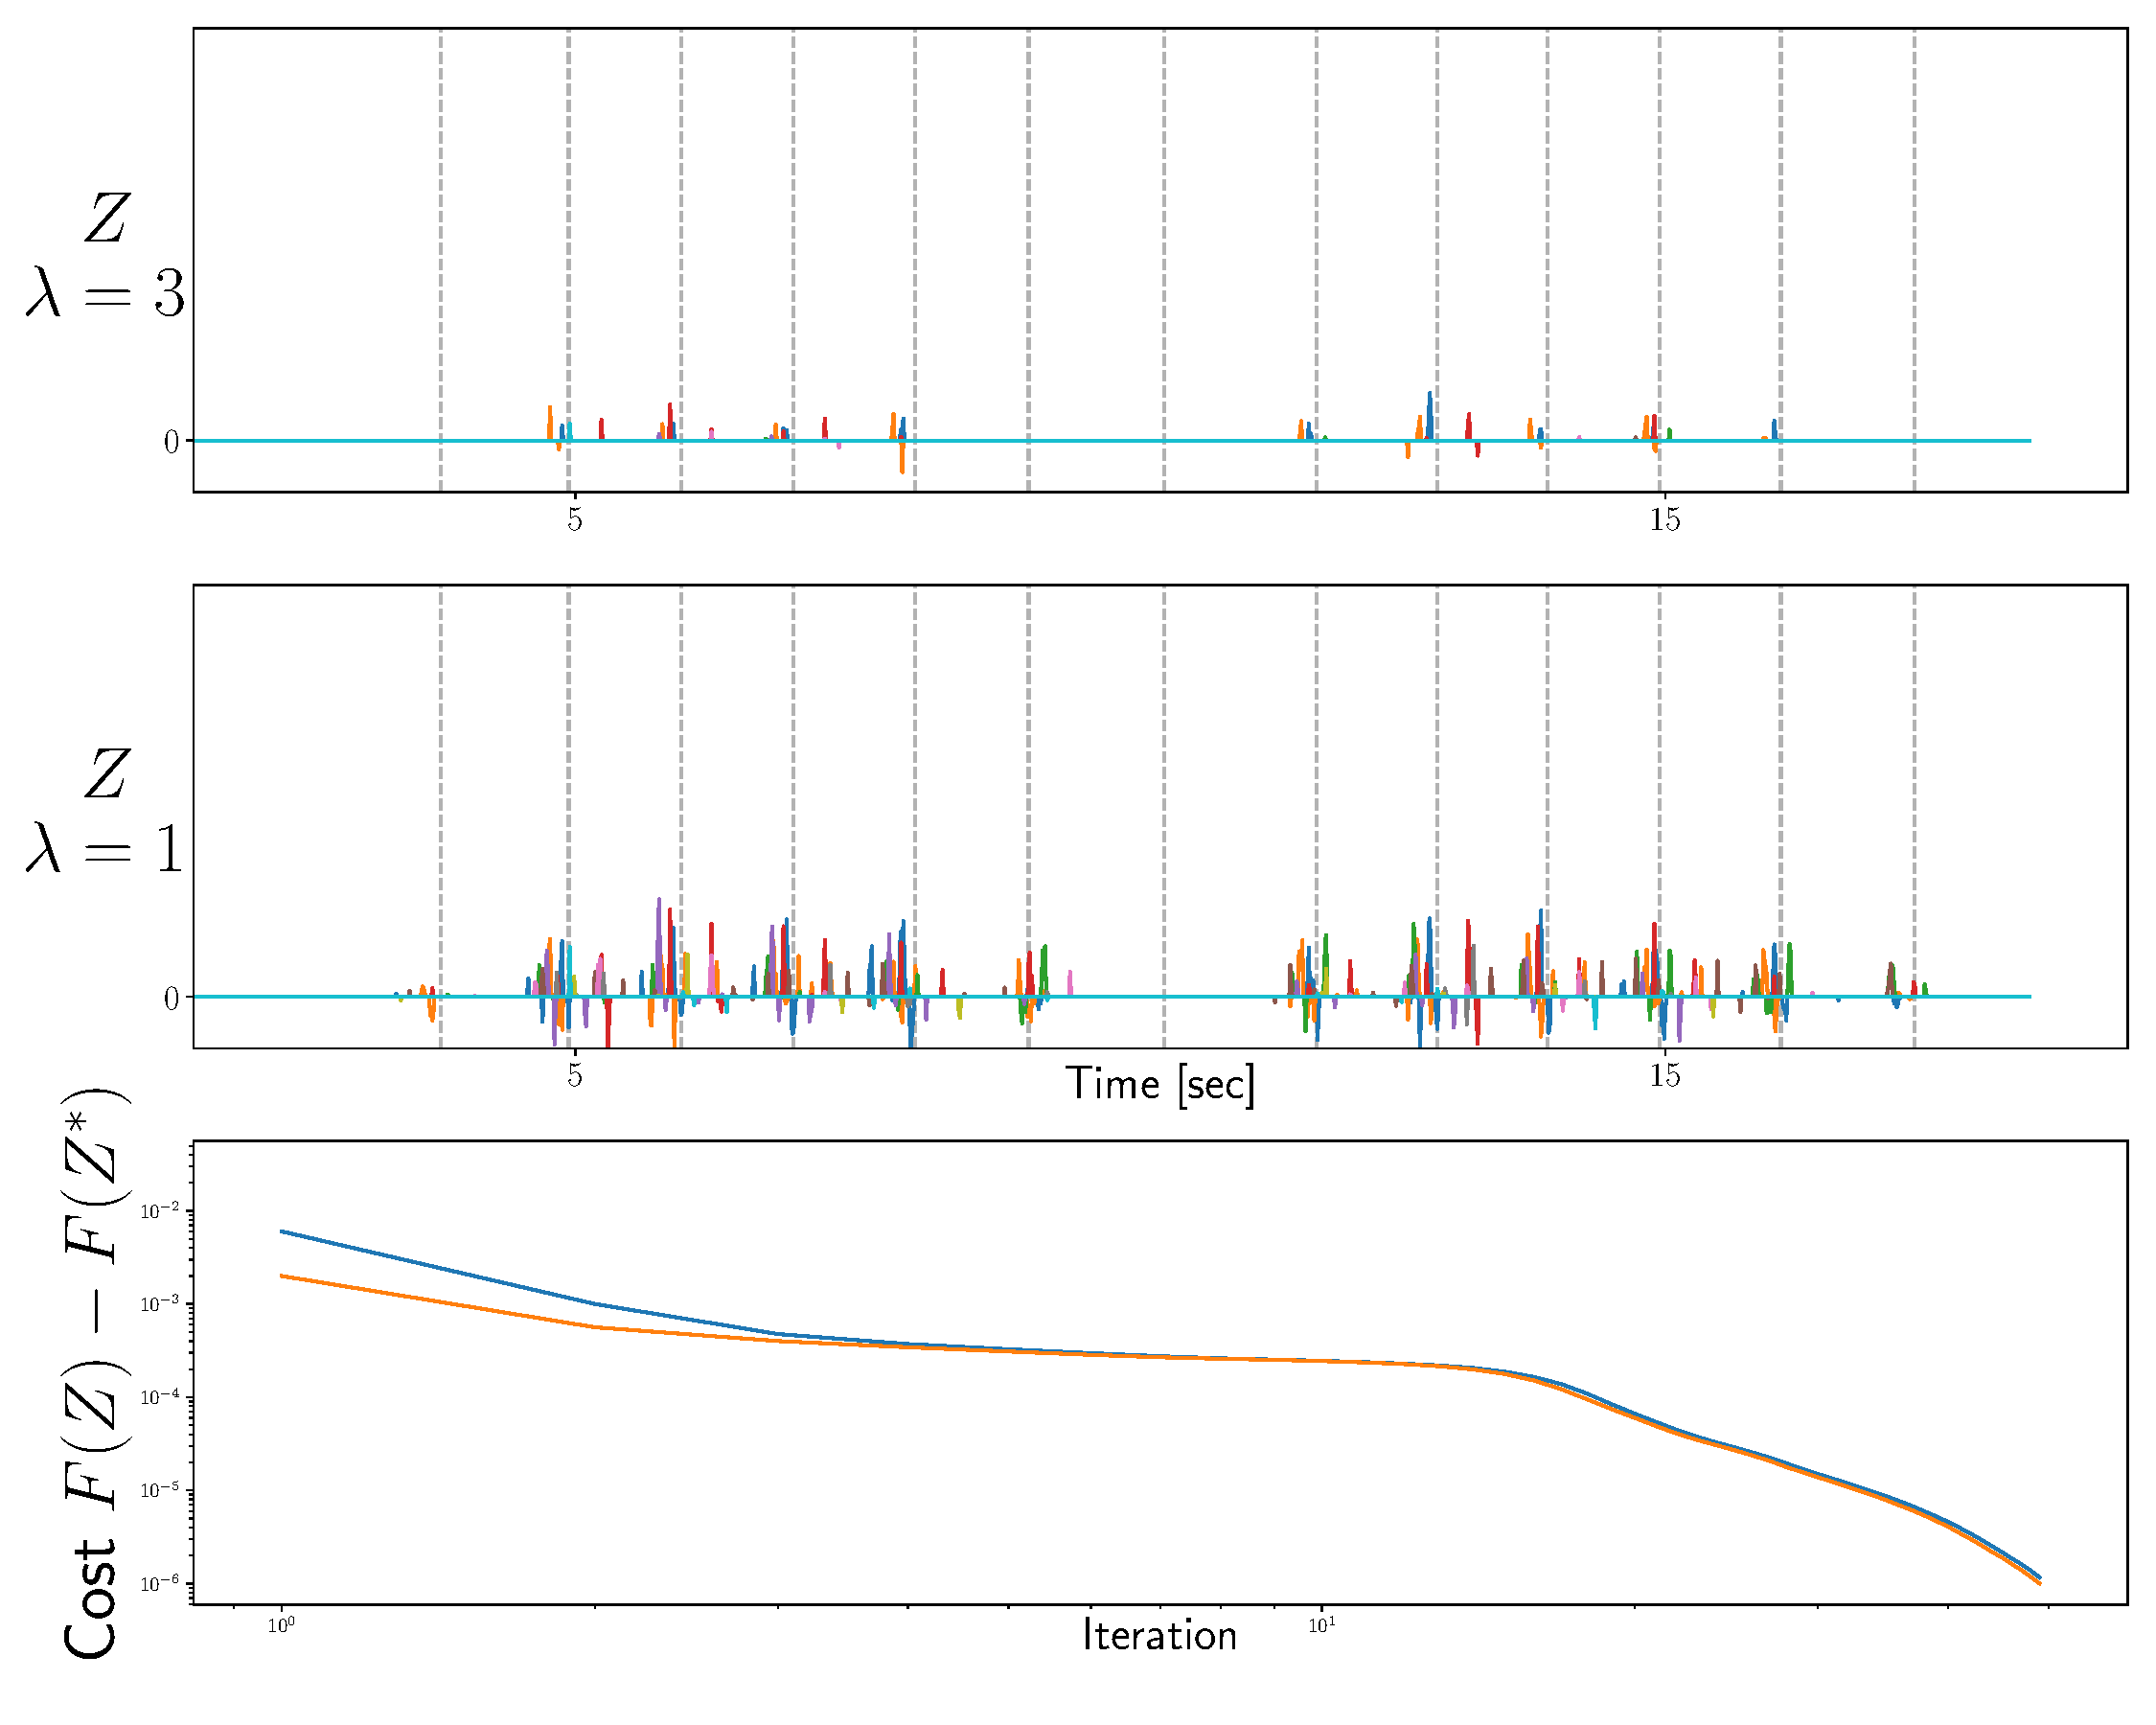
\includegraphics[width=.8\textwidth]{csc_random_annex}	
\end{frame}

%===========================================================================
\subsection{FacNet}
%===========================================================================


\begin{frame}{Related works}

\begin{itemize}\itemsep2em
	\item \cite{Giryes2016}: Propose the inexact projected gradient descent and conjecture that LISTA accelerate the LASSO resolution by learning the sparsity pattern of the input distribution.
	\item \cite{xin2016maximal}: Study the Hard-thresholding Algorithm and its
	capacity to recover the support of a sparse vector.\\
	The paper relax the RIP conditions for the dictionary.
\end{itemize}
\end{frame}


\begin{frame}{Generic Dictionaries}
	\vskip2em
	A dictionary $D \in \Rset^{p\times K}$ is a generic dictionary when its columns
	$D_i$ are drawn uniformly over the $\ell_2$ unit sphere $\mathcal S^{p-1}$.


\end{frame}
\begin{frame}{Theorem (Generic Acceleration)}
	\vskip1em
	In \textbf{expectation over the generic dictionary} $D$, the factorization algorithm using a
		diagonally dominant matrix $A\subset\mathcal E_\delta$, has better performance for
		iteration $q+1$ than the normal ISTA iteration -- which uses the identity -- when
		\[
			\lambda\E[z]{\|z^{(q+1)}\|_1+\|z^*\|_1}
				\le \sqrt{\frac{K(K-1)}{p}} \underbrace{\E[z]{\|z^{(q)}-z^*\|_2^2}
				}_{\substack{\text{expected resolution}\\\text{at iteration $q$ }}}
		\]

	\vskip2em
	FacNet can improve the performances compared to ISTA when this is verified.
\end{frame}



\begin{frame}{L-FISTA}
	\centering
	\vskip4em
	\inputTikZ{.65}{lifsta_tikz}
	\vskip2em
	Network architecture for L-FISTA.
    
\end{frame}
\begin{frame}
	\centering
	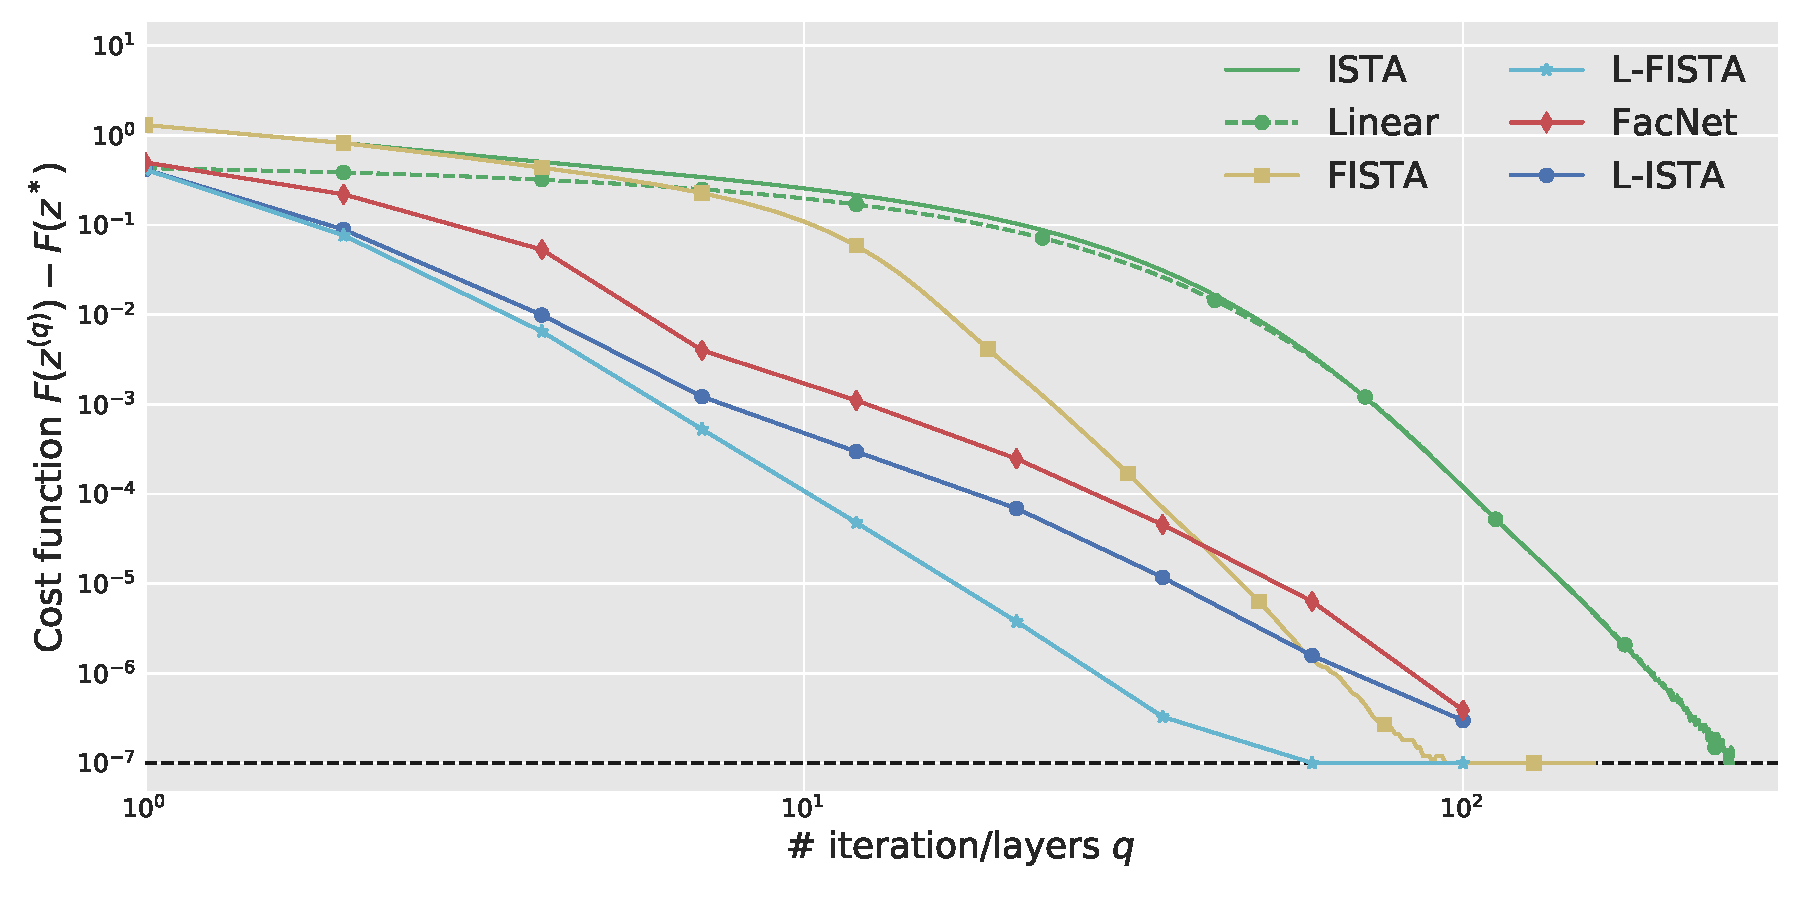
\includegraphics[width=\textwidth]{curve_sparse005_seaborn}
    Evolution of the cost function $F(z^{(q)}) - F(z^*)$ with the number
   	of layers/iterations $q$ with a denser model
\end{frame}
\begin{frame}

	\twocols{
		\centering
		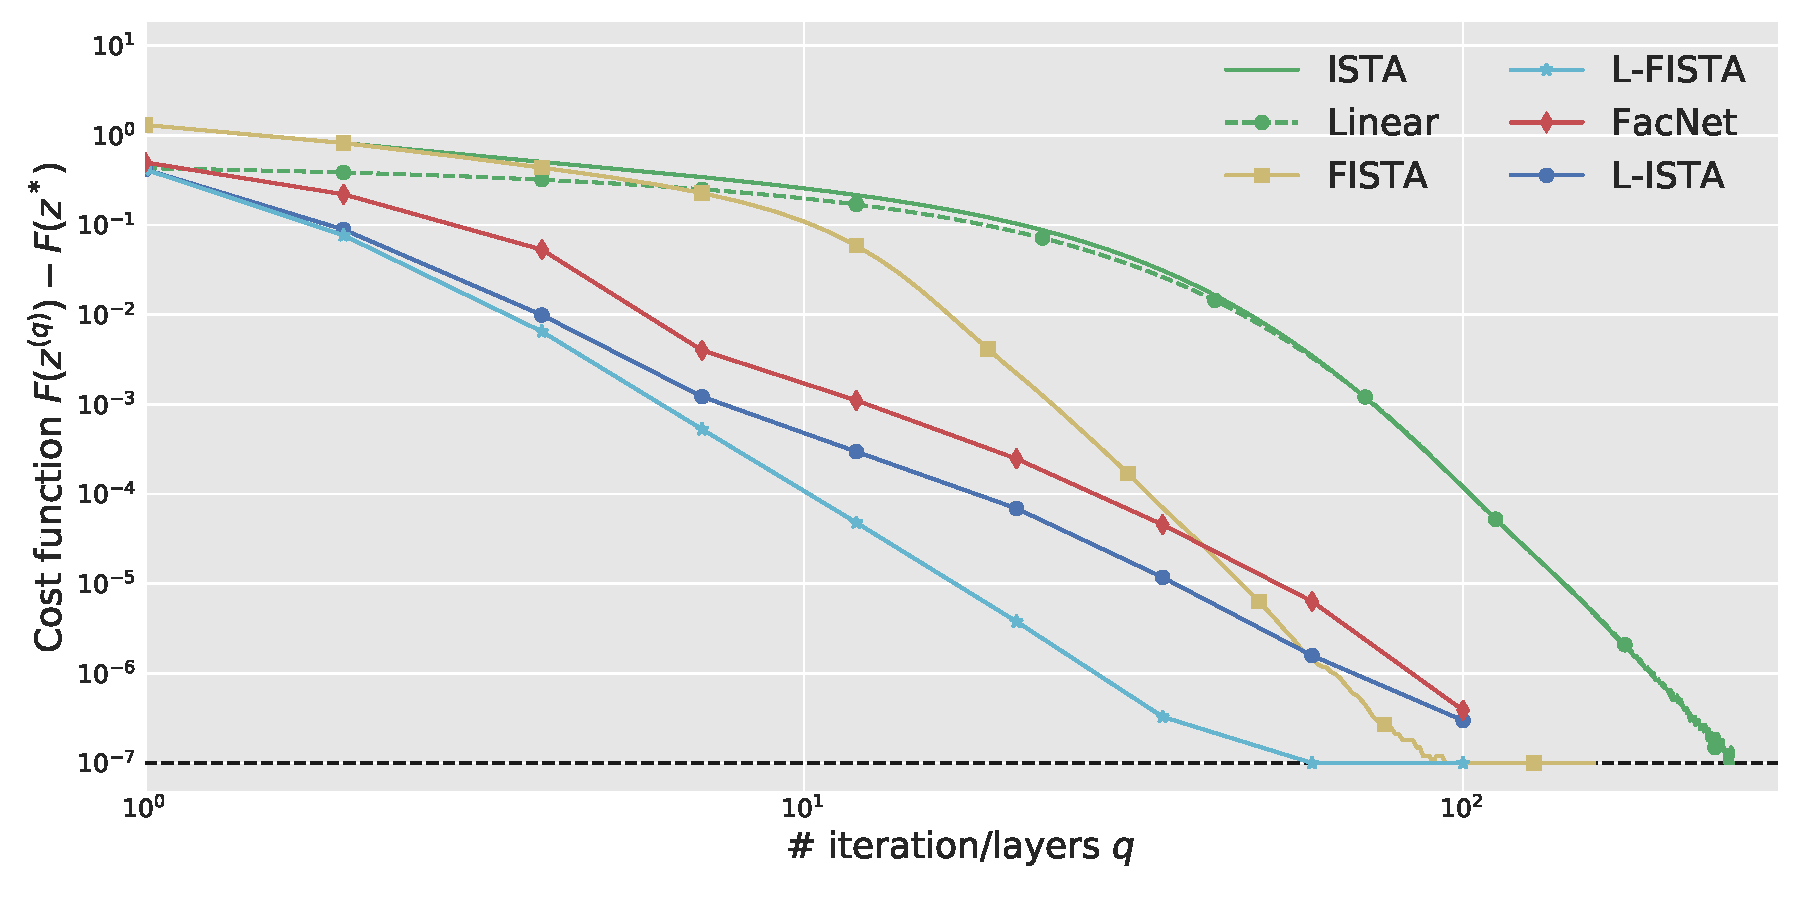
\includegraphics[width=\textwidth]{curve_sparse005_seaborn}\\
		$\rho = {}^1/_{20}$.\\[1em]

		Evolution of the cost function $F(z^{(q)}) - F(z^*)$ with the number
	   	of layers/iterations $q$ with a denser model

	}{
		\centering
		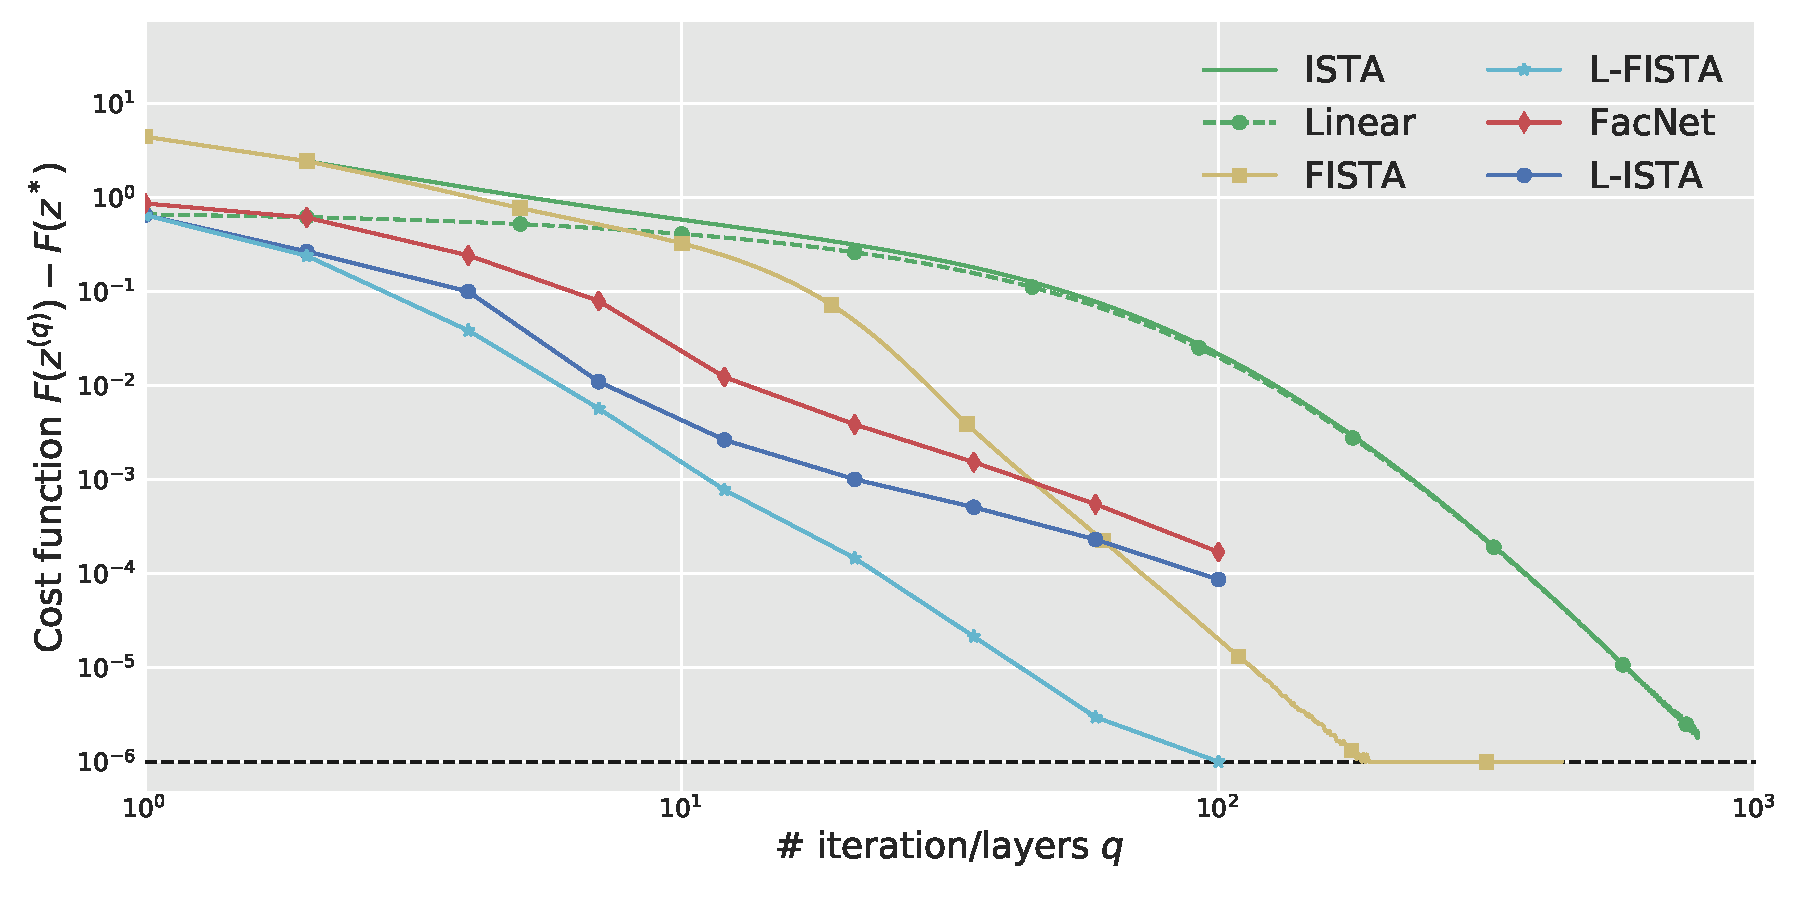
\includegraphics[width=\textwidth]{curve_sparse02_seaborn}\\
		$\rho = {}^1/_{4}$.\\[1em]
		Evolution of the cost function $F(z^{(q)}) - F(z^*)$ with the number
	   	of layers/iterations $q$ with a denser model
	}
\end{frame}


\begin{frame}{PASCAL 08}
{
	\vskip1em
	Sparse coding for the PASCAL 08 datasets over the Haar wavelets family.\\[1em]
	\emph{Patch size:} 8x8;~~~$K = 267$;~~~  \emph{train/test:} 500/100\\[1em]
	\centering
	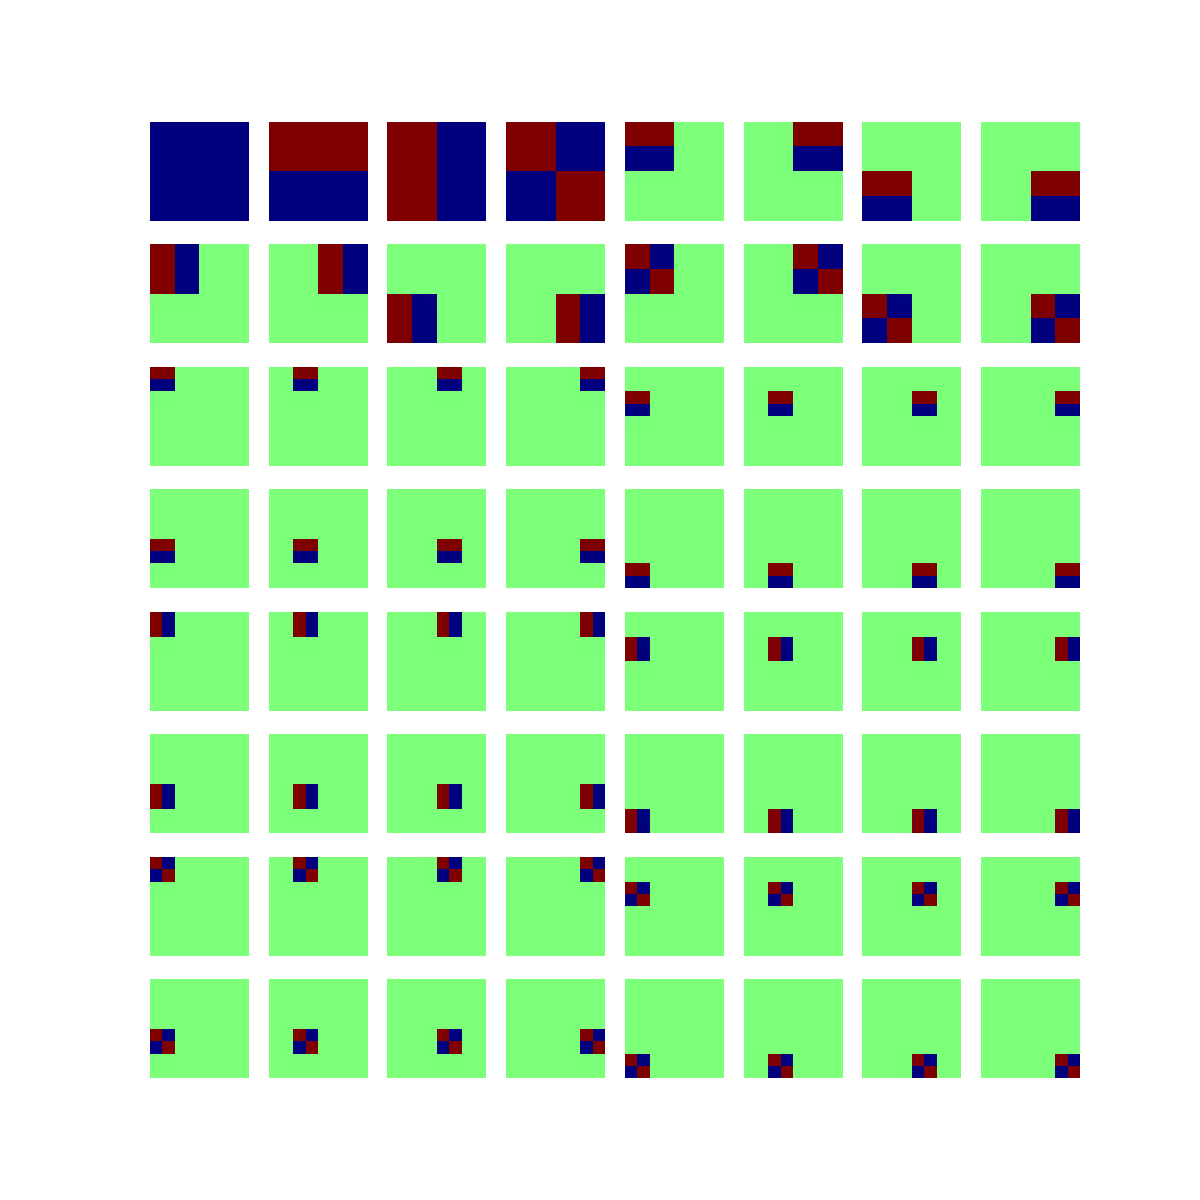
\includegraphics[width=.6\textwidth, trim={5em 4em 4em 4em}, clip]{Wavelets}\\
}{
	\vskip5em
    \centering
    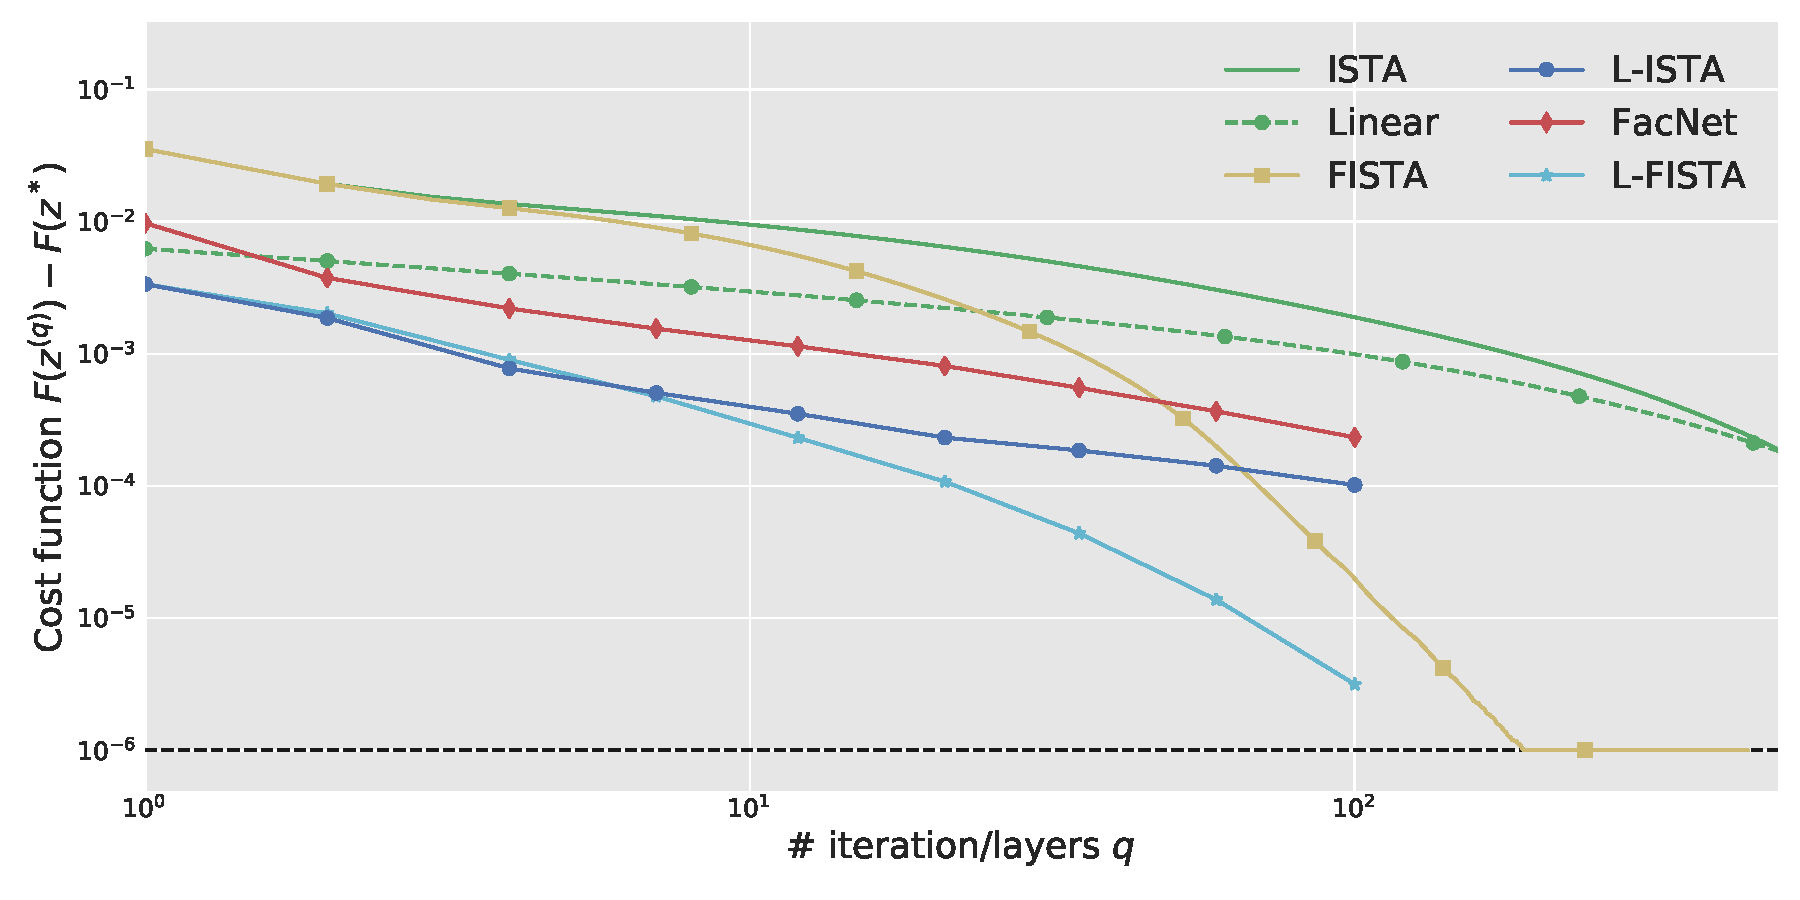
\includegraphics[width=\textwidth]{curve_images_seaborn}\\
     Evolution of the cost function $F(z^{(q)})-F(z^*)$ with the number of layers
     or the number of iteration $q$ for Pascal VOC 2008.
}
\end{frame}


\begin{frame}{MNIST}
	\vskip1em
	Dictionary $D$ with $K=100$ atoms learned on 10 000 MNIST samples (17x17) with dictionary learning.
	LISTA trained with MNIST training set and tested on MNIST test set.\\[1em]
{
    \centering
    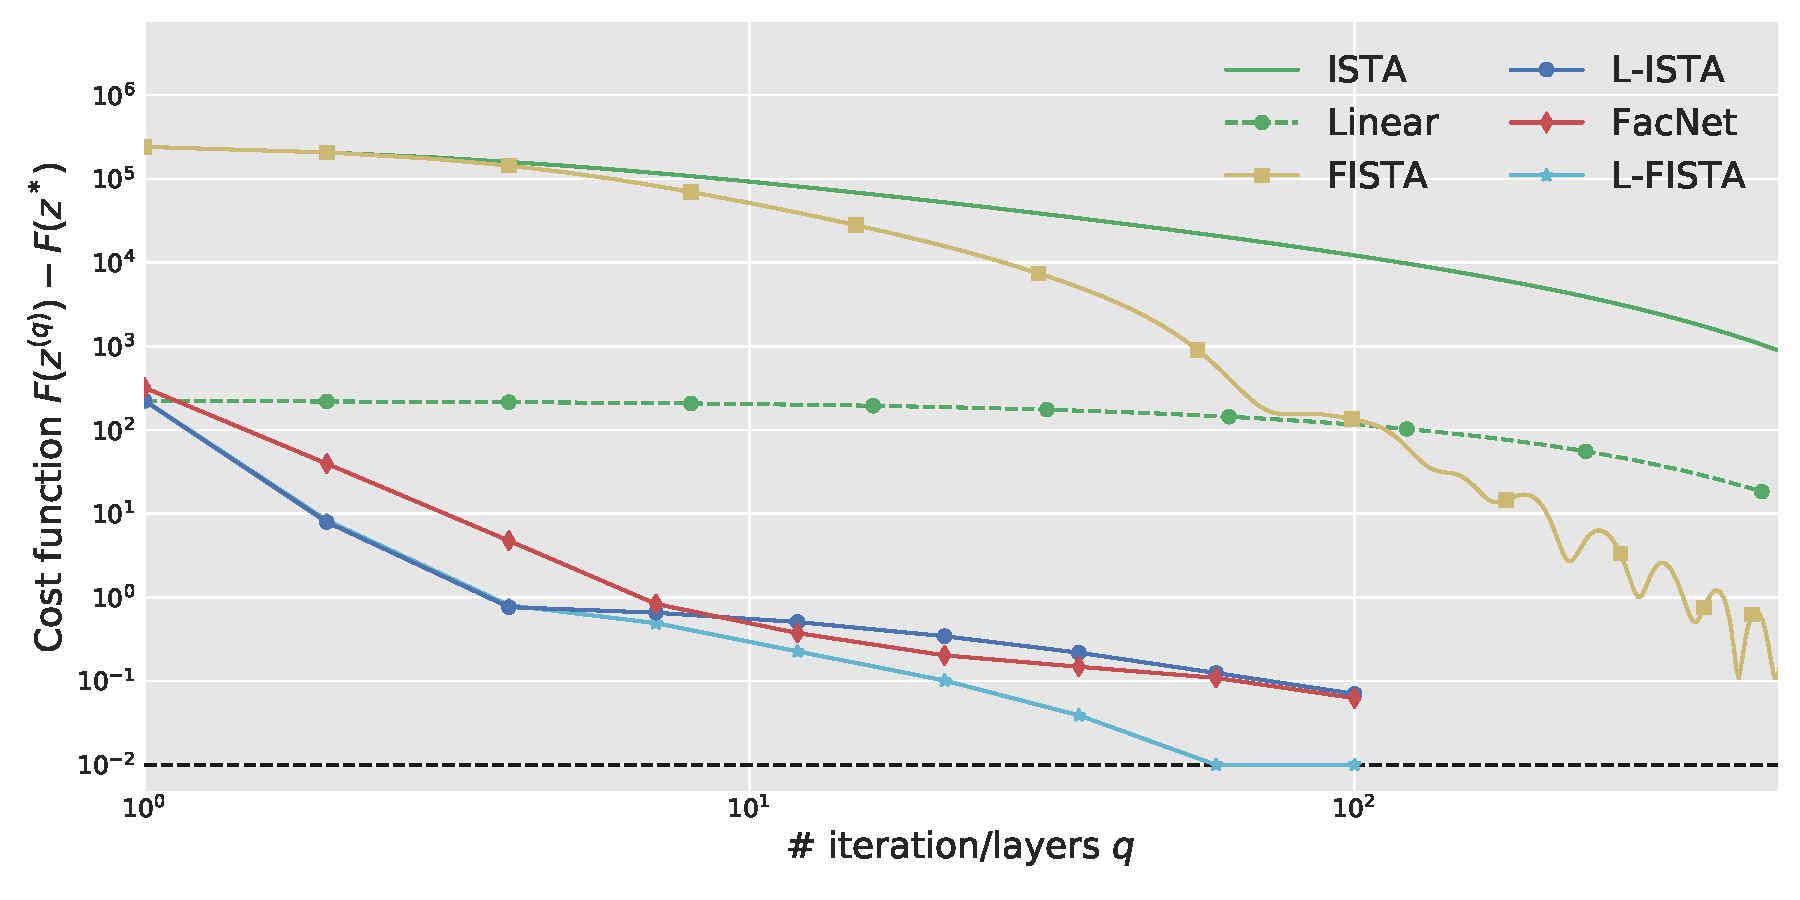
\includegraphics[width=\textwidth]{curve_mnist_seaborn}\\
     Evolution of the cost function $F(z^{(q)})-F(z^*)$ with the number
     of layers or the number of iteration $q$ for MNIST.
}
\end{frame}

\begin{frame}{Adversarial dictionary}
\vskip2em
The dictionary is constructed such that it eigen-vectors are sampled from the
Fourier basis, with
\[
D_{k, j} = e^{-2i\pi k \zeta_j}
\]
for a random subset of frequencies
\[
\left \{ \zeta_i \right \}_{0\le i \le p} \sim \mathcal U \left\{\frac{m}{K}; 0 \le m \le \frac{K}{2}\right\}
\]
Diagonalizing $B$ implies large deformation of the $\ell_1$-norm. 

\end{frame}



%====================================================================
\subsection{DICOD}
%====================================================================

\begin{frame}{Finishing the process in a distributed environment}


	Non trivial point: {\bf How to decide that the algorithm has converged?}\\[2em]
	
	\begin{itemize}\itemsep2em\itemindent1em
		\item Neighbors paused is not enough!
		\item Define a master 0 and send probes.\\
			\hskip3em Wait for $M$ probes return.
		\item Uses the notion of message queue and network flow.\\
			\hskip3em Maybe we can have better way?
	\end{itemize}
	
	
\end{frame}


\begin{frame}
\frametitle{Numerical Experiments}


\definecolor{fista}{RGB}{192,192,0}
\definecolor{rcd}{RGB}{0,128,0}
\definecolor{cd}{RGB}{255, 0, 0}
\definecolor{dicod}{RGB}{0,0,255}

Test on long signals generated with Bernoulli-Gaussian
coding signal $Z$ and a Gaussian dictionary $\pmb D$.
Fixed $K = 25$, $W = 200$ and $T = 600*W$,\\[1em]

\textbf{Algorithms implemented for benchmark}
\begin{itemize}
    \item {\color{cd} Coordinate Descent} (CD) \\\mycite{Kavukcuoglu2013}
    \item {\color{rcd} Randomized Coordinate Descent} (RCD) \\\mycite{Nesterov2010}
    \item Fast Convolutional Sparse Coding (FCSC)\\\mycite{Bristow2013}
    \item {\color{fista}Fast Ierative Soft-Thresholding Algorithm (FISTA)} \\\mycite{Chalasani2013, Wohlberg2016}
    \item {\color{dicod} DICOD with $60$ cores}
\end{itemize}
\end{frame}


\begin{frame}{Numerical convergence}

\centering
\alt<2>{
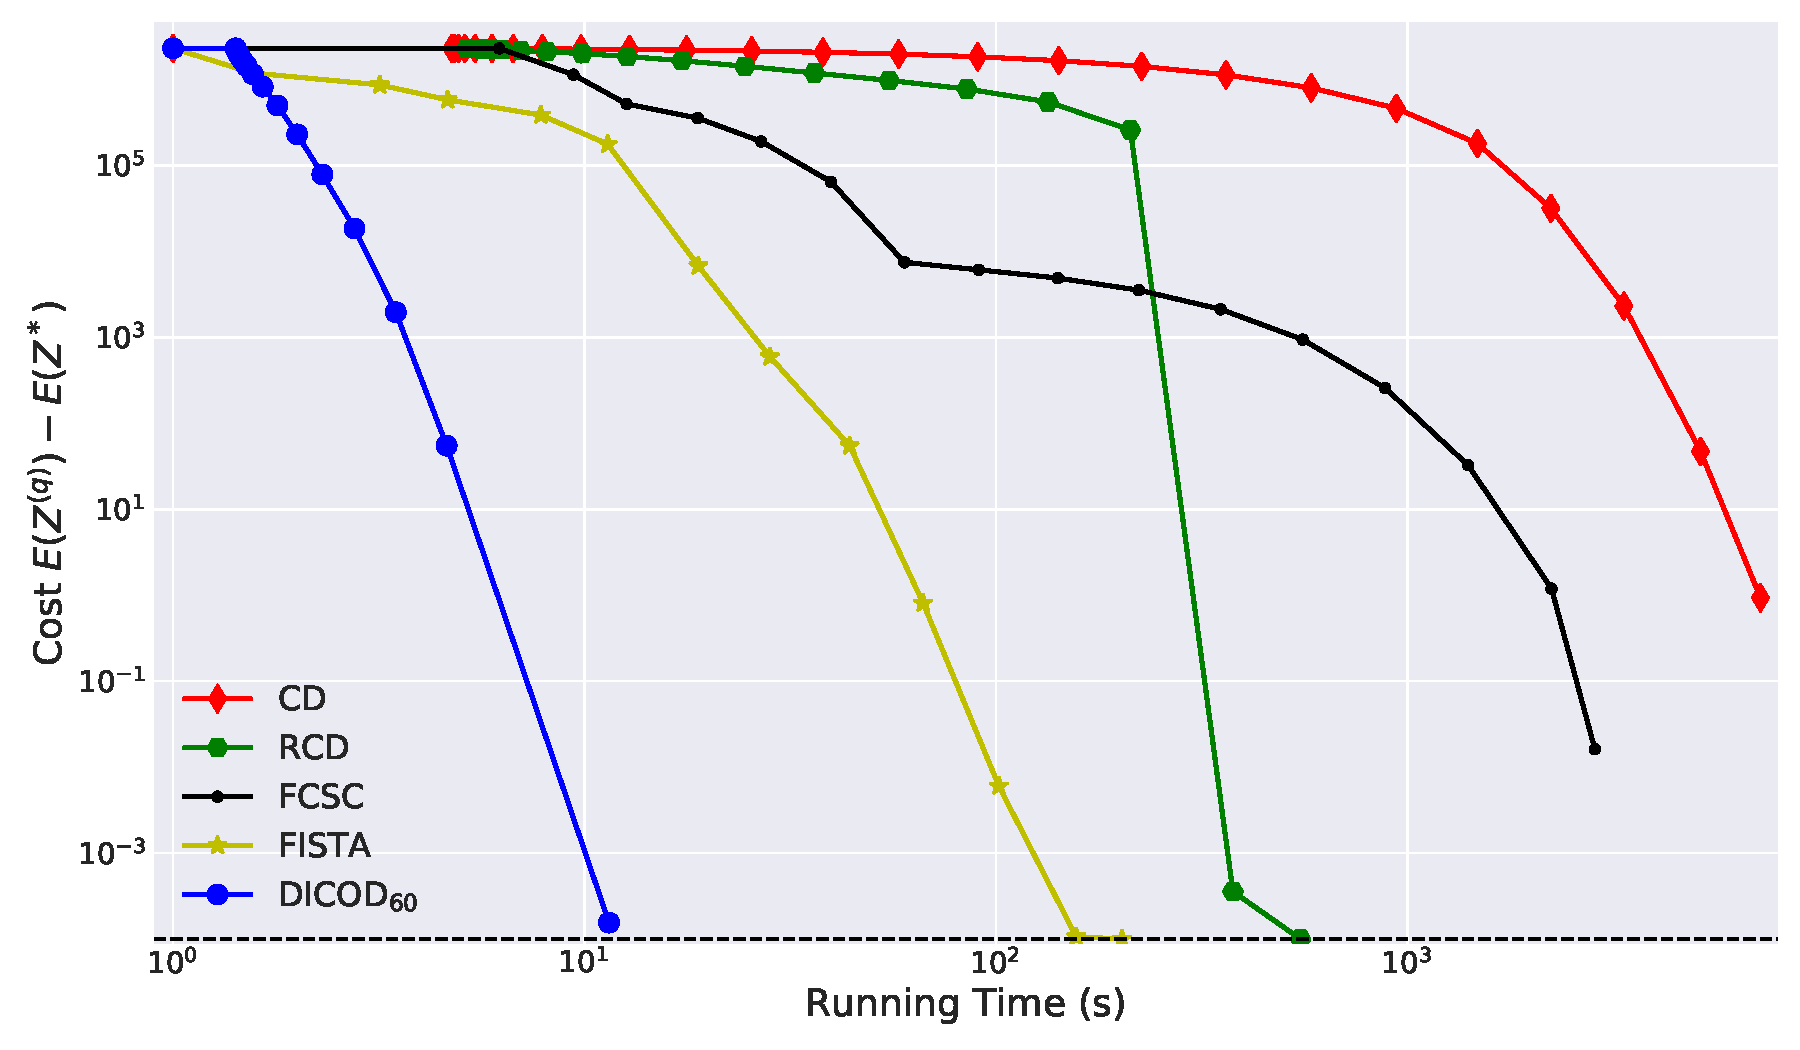
\includegraphics[width=.8\textwidth]{cost_min_seaborn_time}\\
\large Cost as a function of the runtime\\
}{
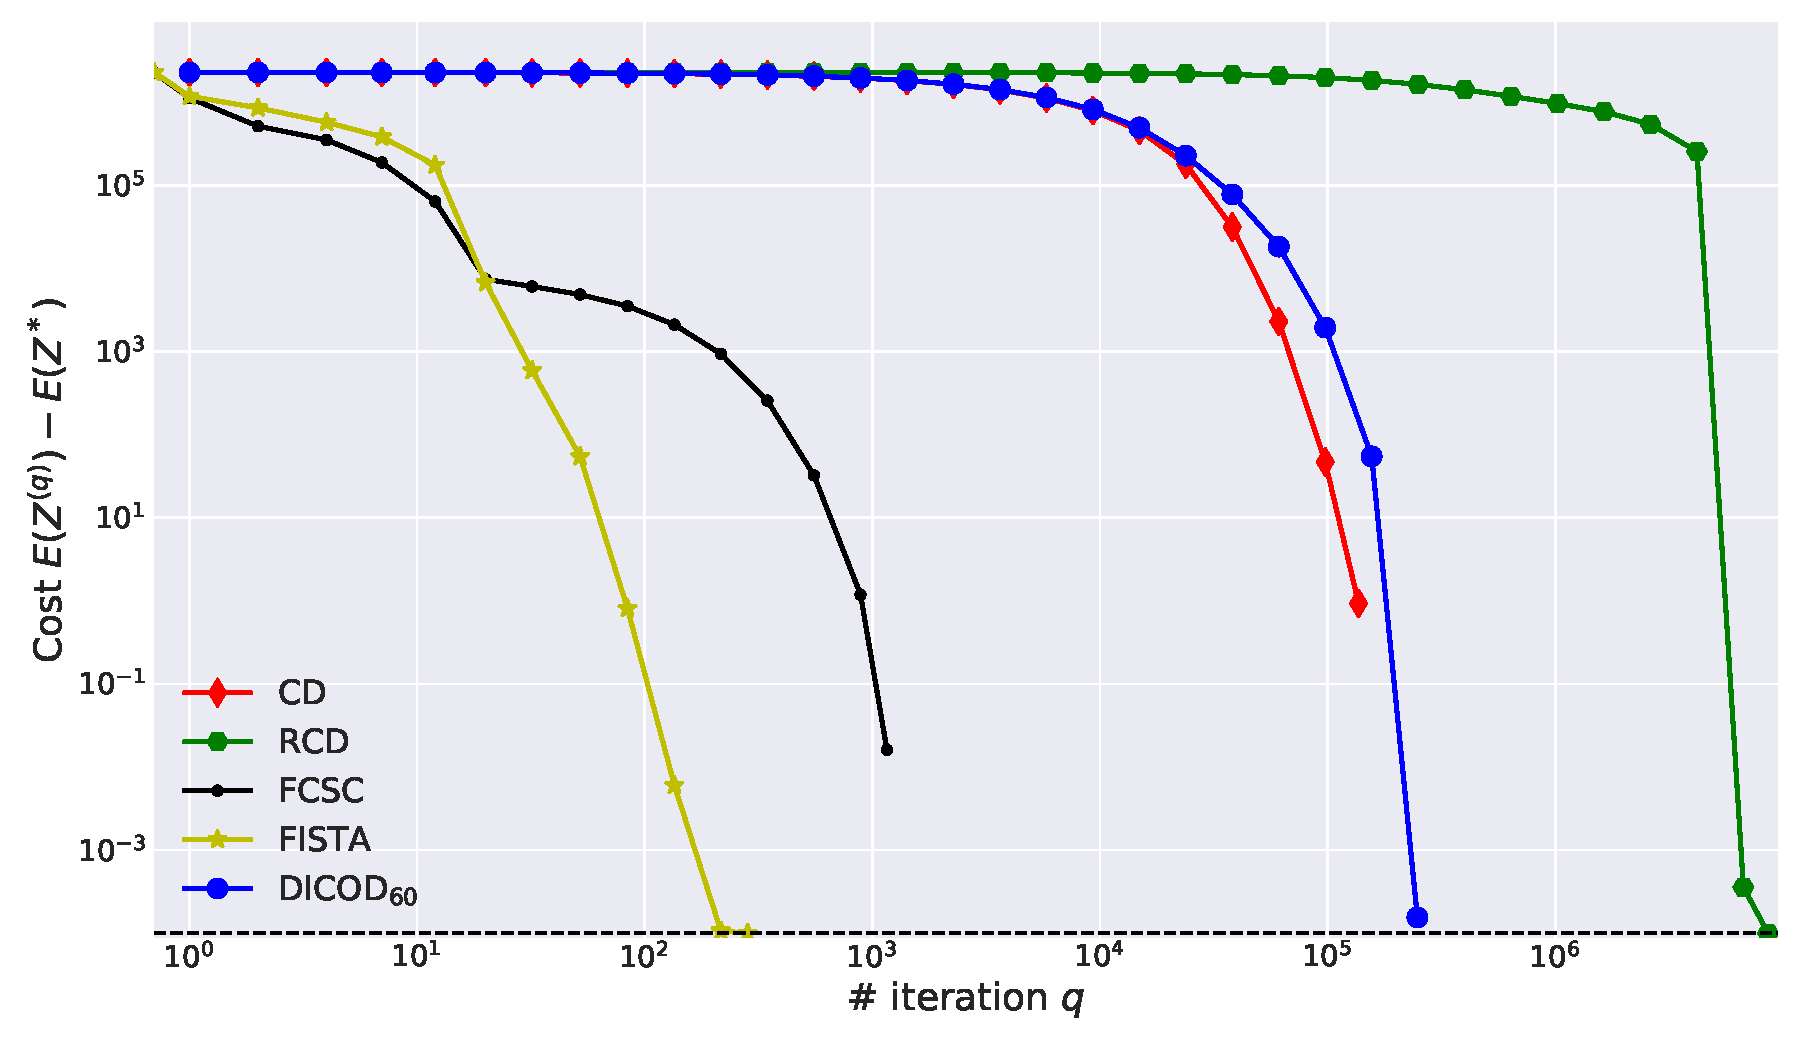
\includegraphics[width=.8\textwidth]{cost_min_seaborn_iter}\\
\large Cost as a function of the iterations\\
}
\end{frame}



\begin{frame}{DICOD: numerical convergence}
	\alt<2>{
		\centering
		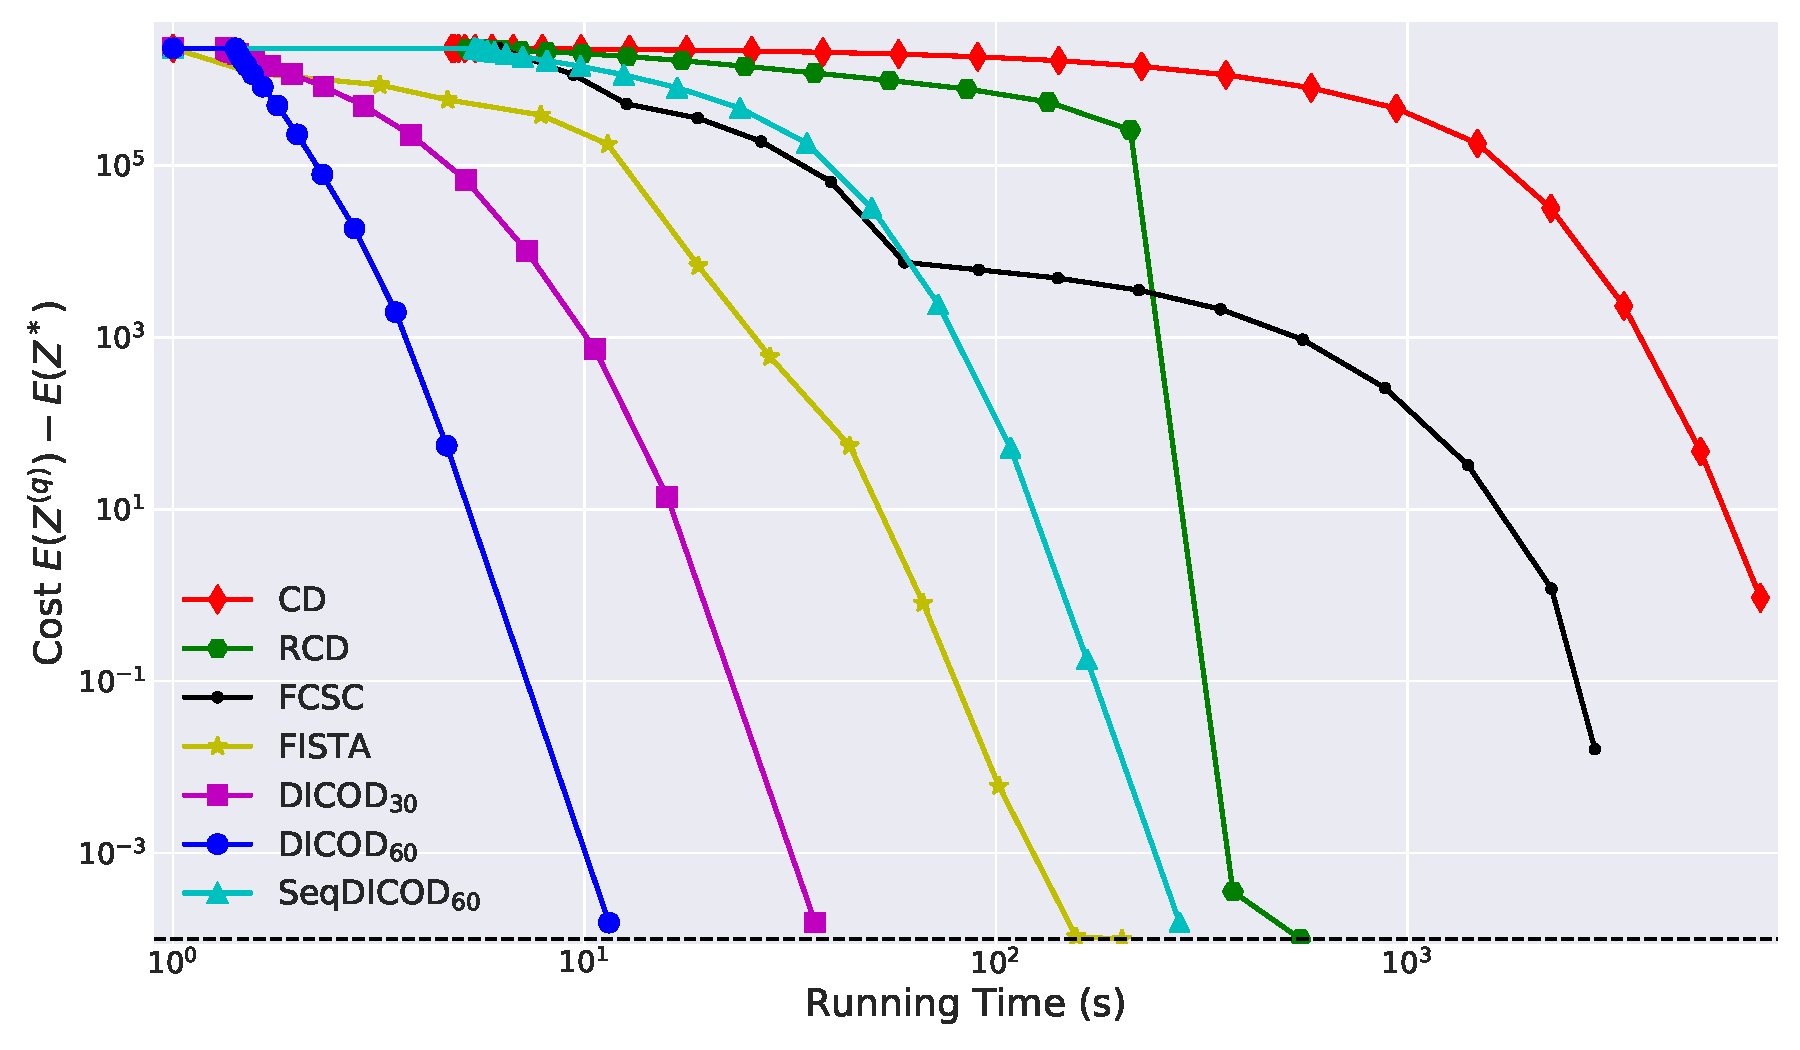
\includegraphics[width=\textwidth]{cost_seaborn_time}\\
		\large Cost as a function of the time
	}{
        \centering
        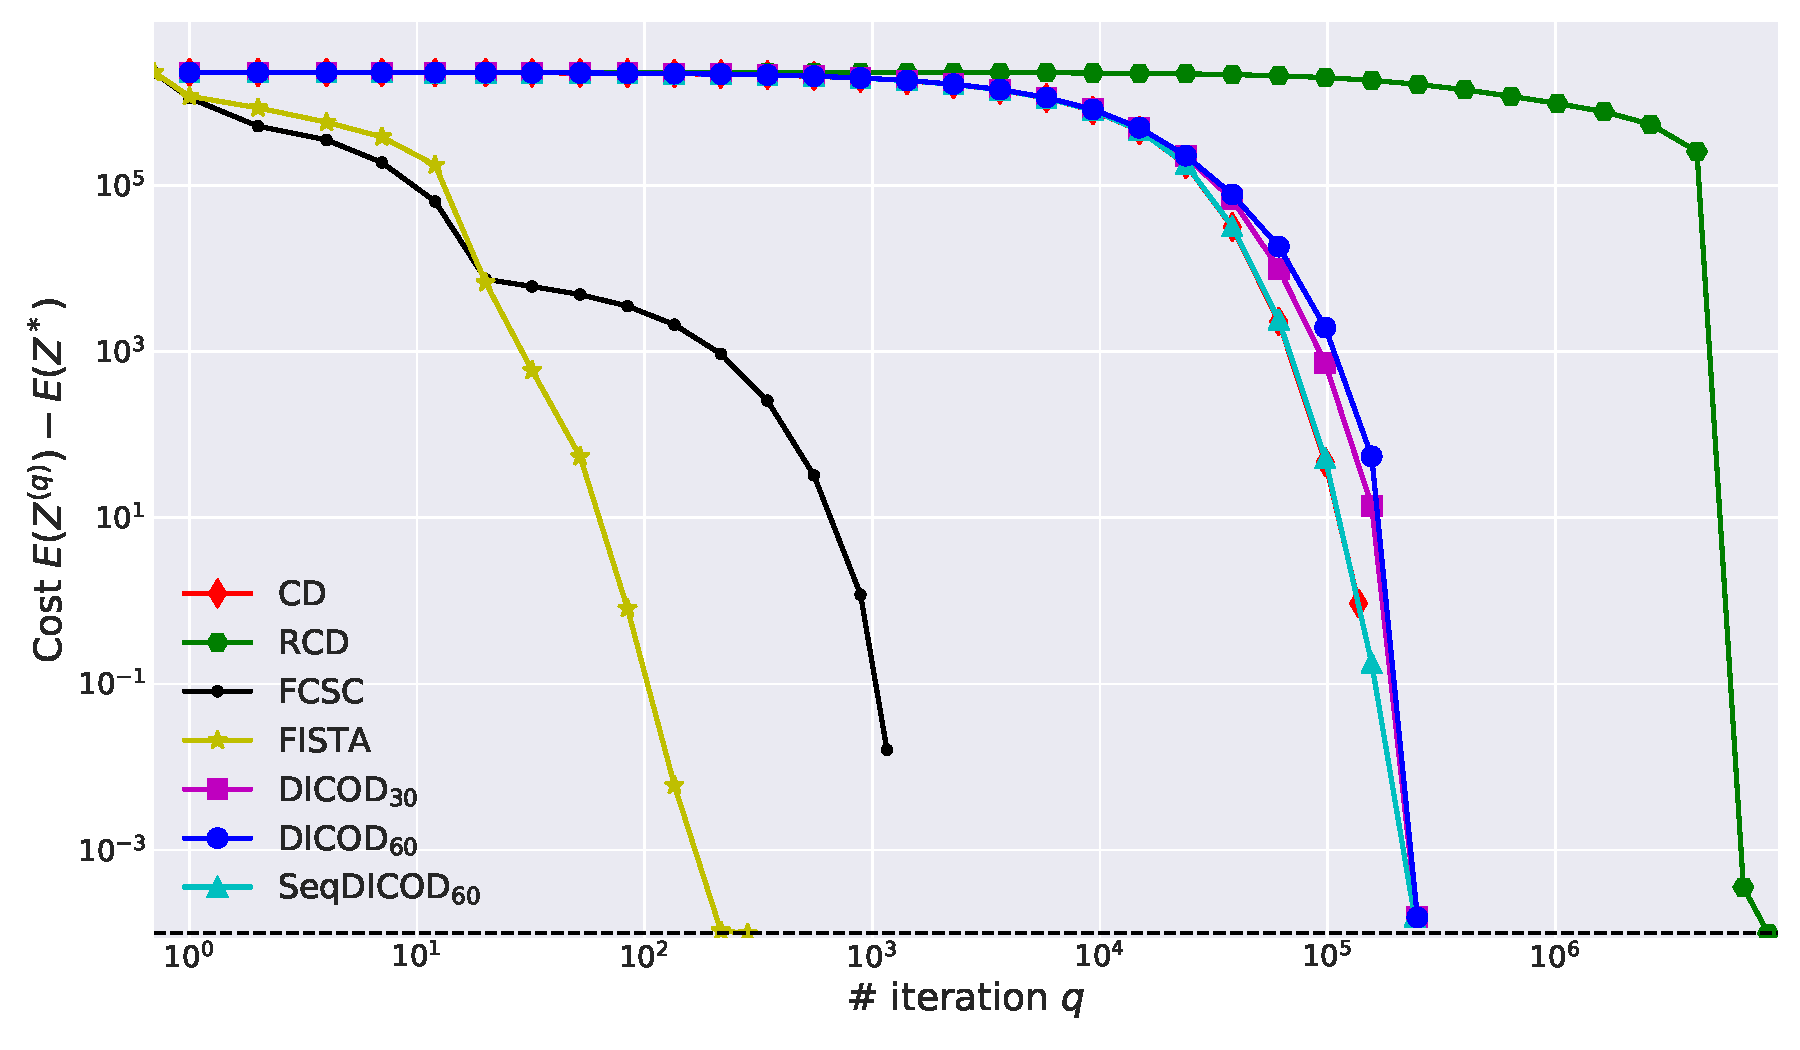
\includegraphics[width=\textwidth]{cost_seaborn_iter}\\
        \large Cost as a function of the iterations
    }
\end{frame}


\begin{frame}{Complexity Analysis}
Two sources of acceleration:\\[1em]
\begin{itemize}\itemsep1em
    \item Perform $M$ updates in parallel,
    \item Each update is computed on a segment of size $\frac{L}{M}$\\
    Iteration complexity of $\bO{K\frac{L}{M}}$ instead of $\bO{KL}$ 
\end{itemize}
\vskip1em
Limitations:
\begin{itemize}
    \item Interfering updates, with probability $\alpha^2 = \left(\frac{WM}{T}\right)^2$
    \[
    \mathbb E[Q_{dicod}] \smeq\underset{\alpha \to 0}{\gtrsim}
    M(1-2\alpha^2M^2 + \mathcal O(\alpha^4M^4))~.
    \]
    \item Cost of the update of $\beta$ in $\bO{KW}$  
\end{itemize}

\end{frame}


\begin{frame}[t]{Soft-Locks \mycite{Moreau2019}}
\vskip2em
{
    \centering
    \inputTikZ{.7}{soft_lock}\\
}

\begin{itemize}[<+->]
    \item Keep track of the value of the optimal update in an extended zone of size $L-1$.
    \item Select an update candidate with LGCD.
    \item If it is in the interfering zone, compare the value of the update with the value potential updates in the other worker.
    \item Only perform the udpate if it is larger than the other update.
\end{itemize}

\only<5>{\strongpoint{Give an update order asynchronously.}}

\end{frame}

\begin{frame}{Images from Hubble Space Telescope}

{\centering
    \alt<2>{
        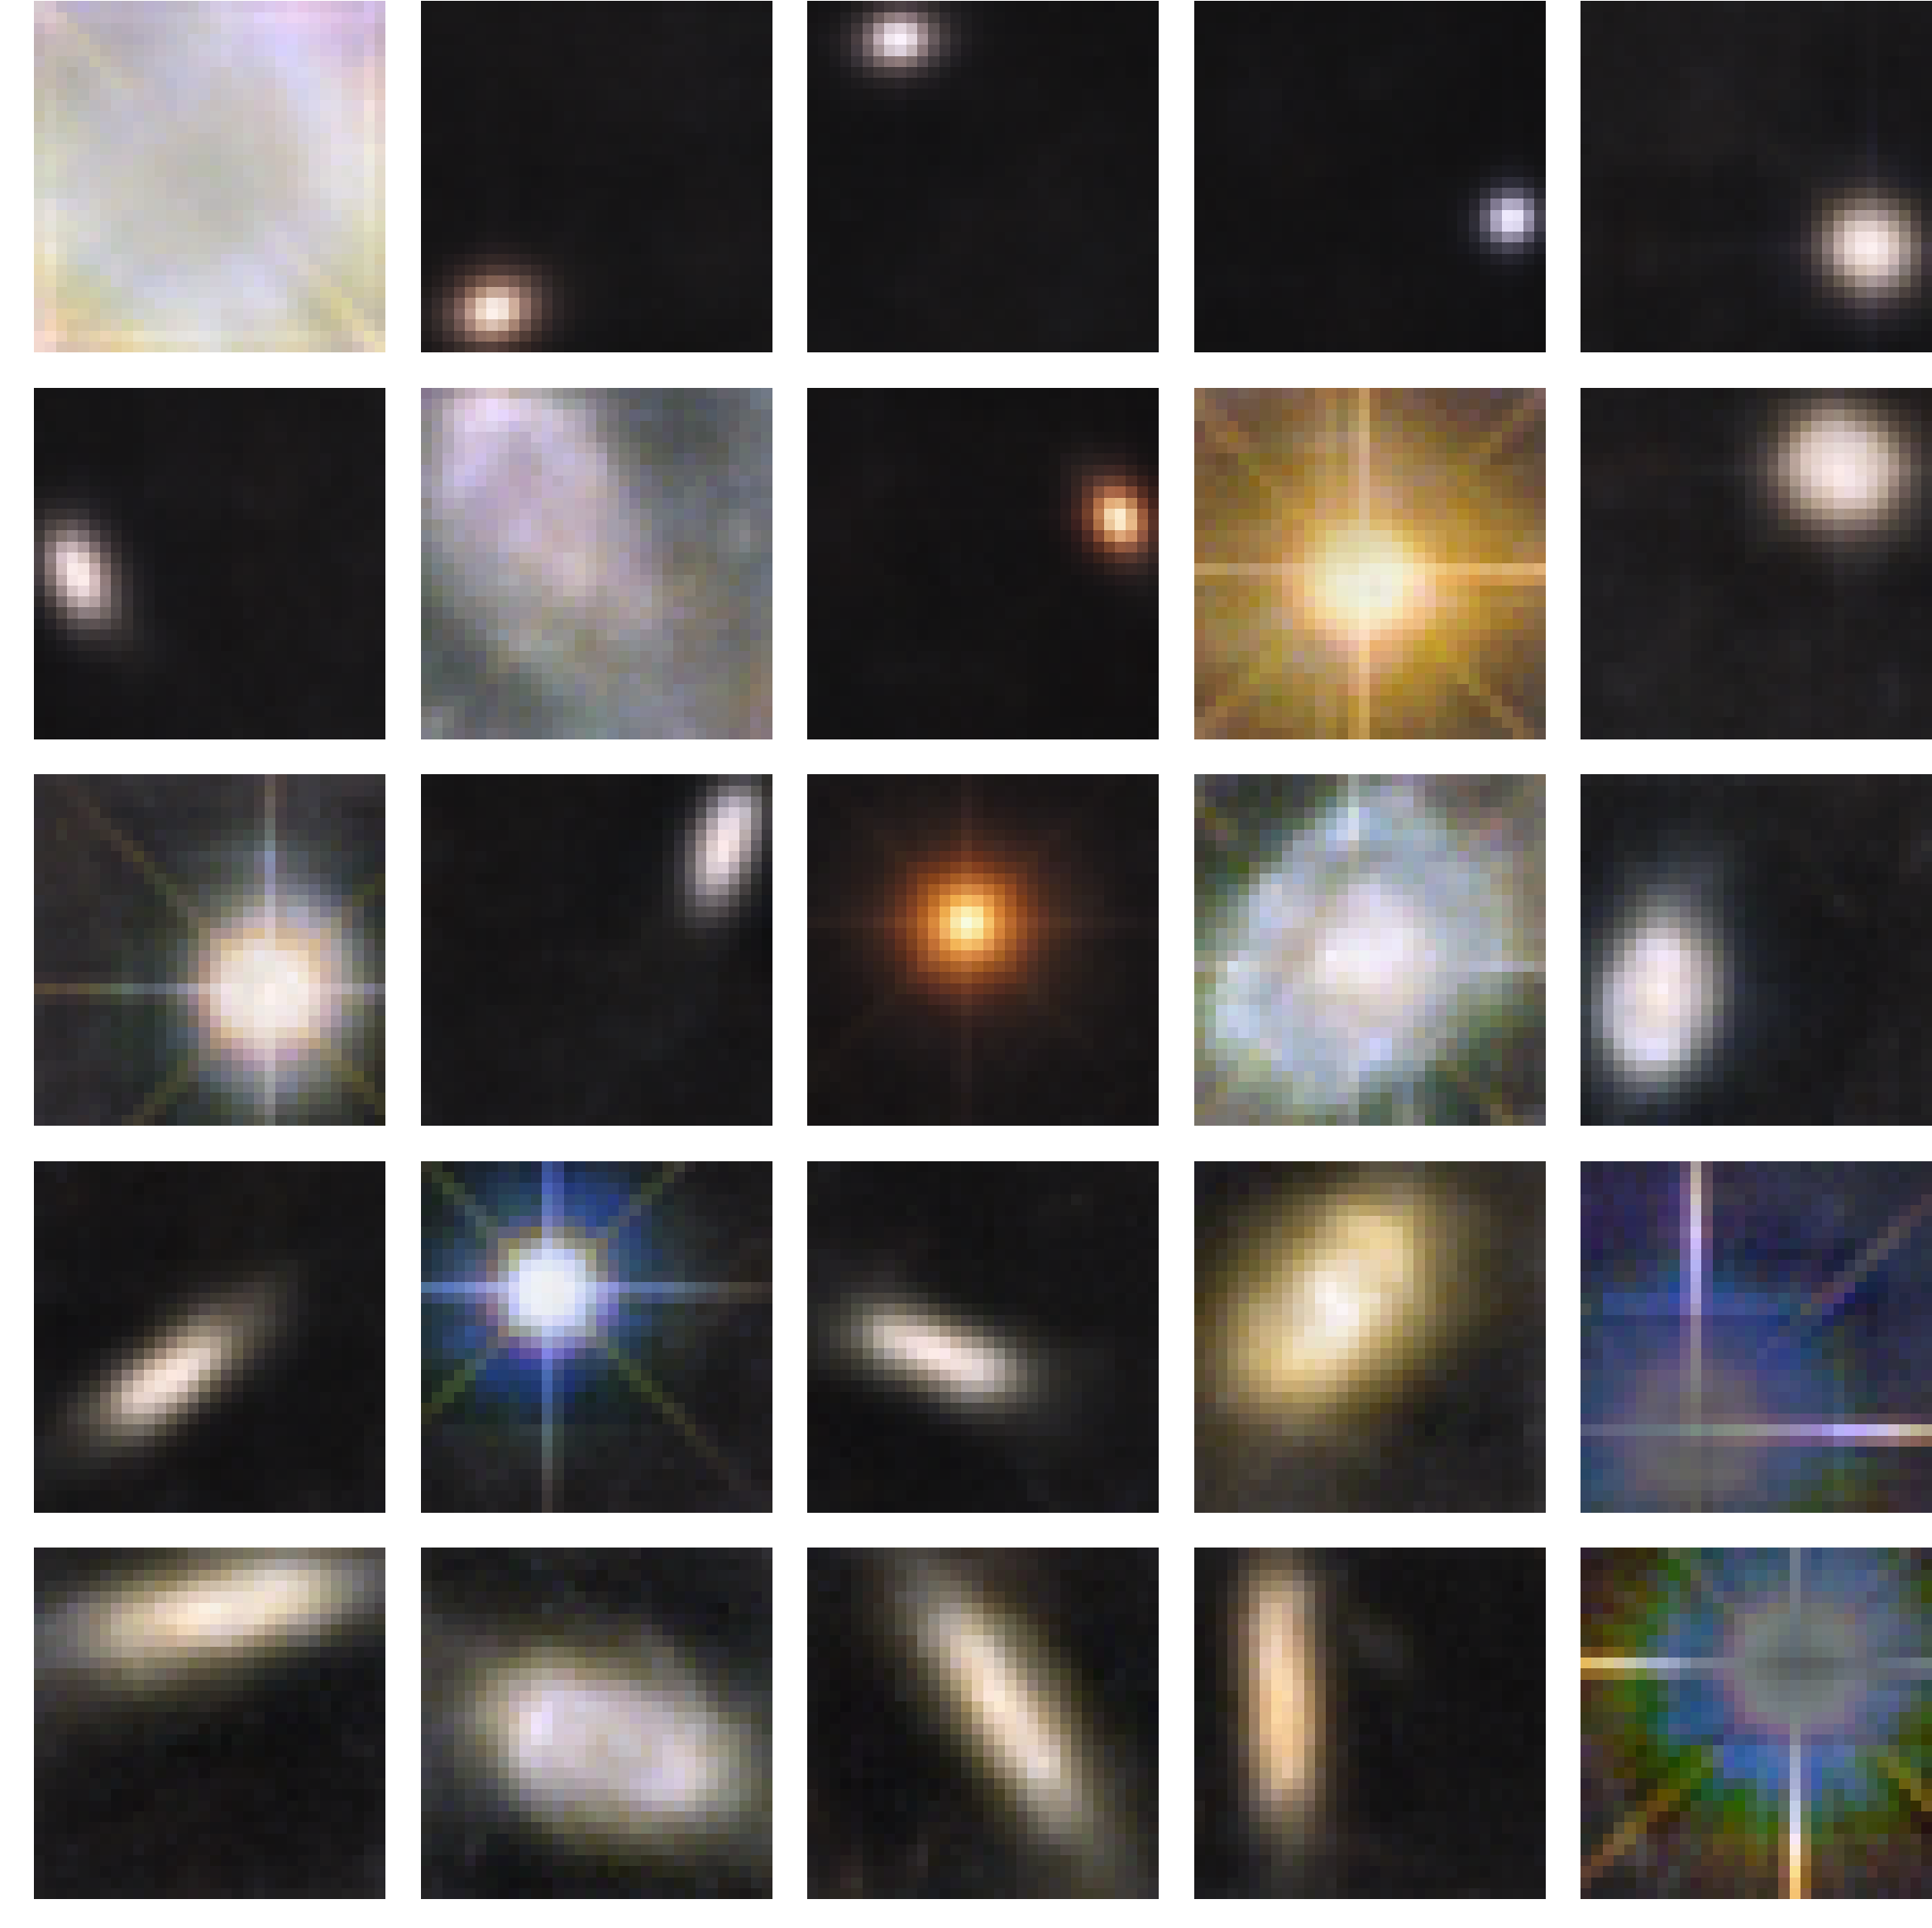
\includegraphics[width=.65\textwidth]{K25_L32_reg0,1_seed42_dicodile_Medium_dict}\\
    }{
        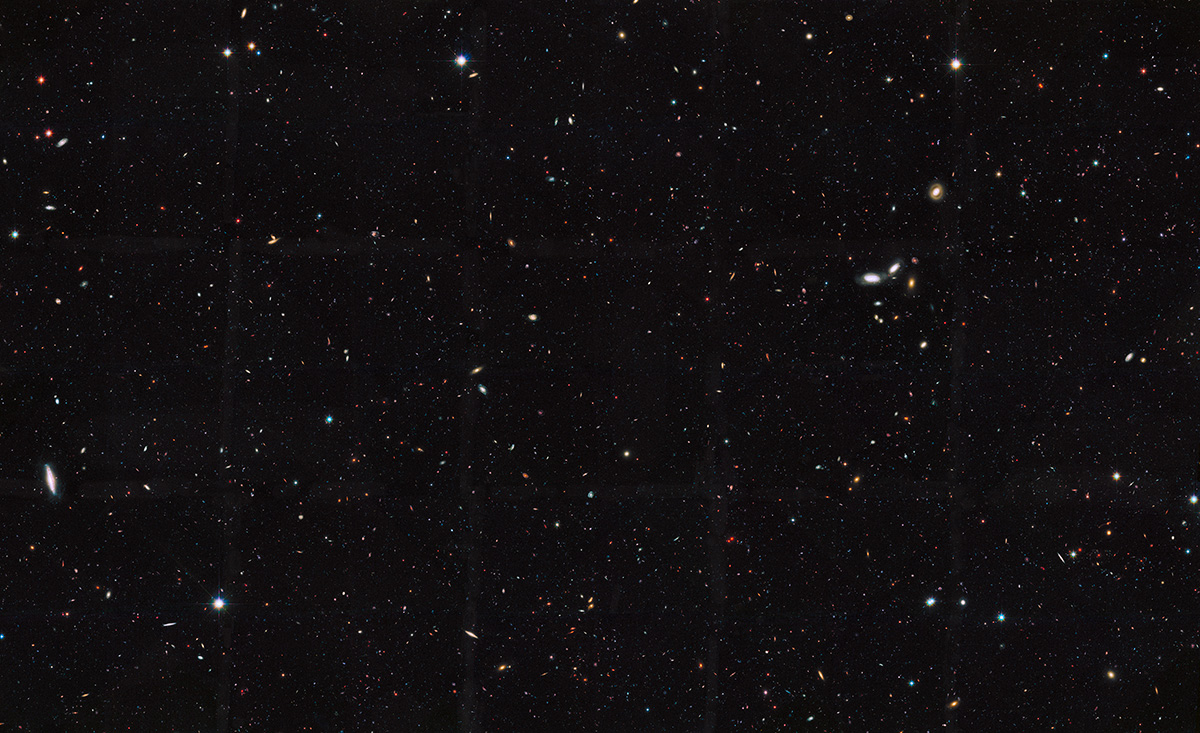
\includegraphics[width=.9\textwidth]{STScI-H-2016-39-a-Small}\\
    }
}
\end{frame}

\section{MultiCSC}



\begin{frame}{Studying brain activity through electromagnetic signals}
\begin{itemize}
    \item Brain (electrical) activity produces an electromagnetic field.
    \item This can be measured with EEG or MEG.
\end{itemize}

\begin{columns}[T]
    \column{.5\textwidth}
    \centering
    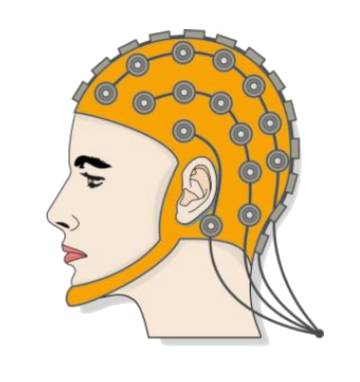
\includegraphics[height=6em]{eeg}\hskip4em
    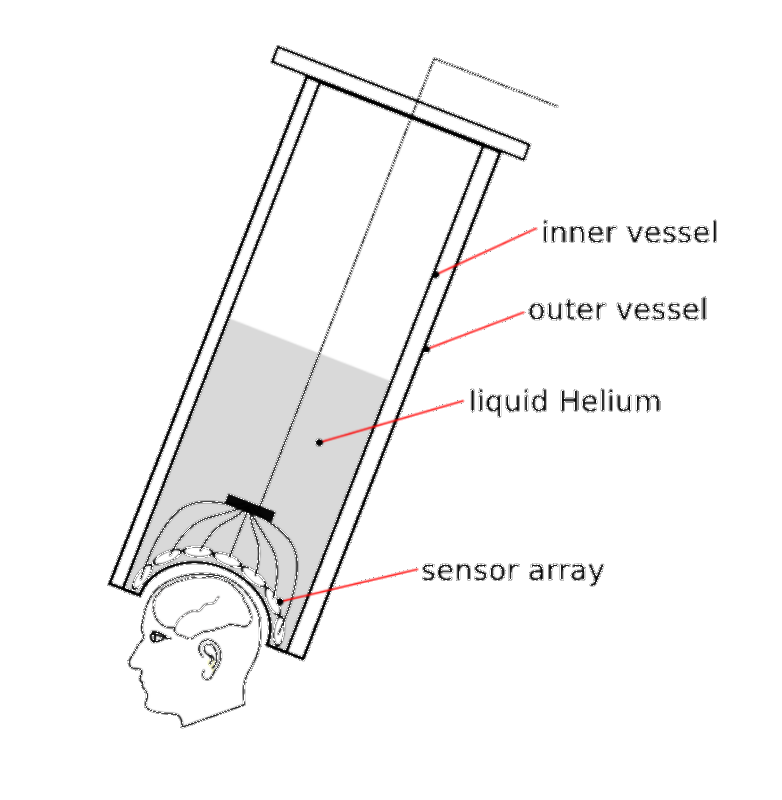
\includegraphics[height=6em]{meg}\\
    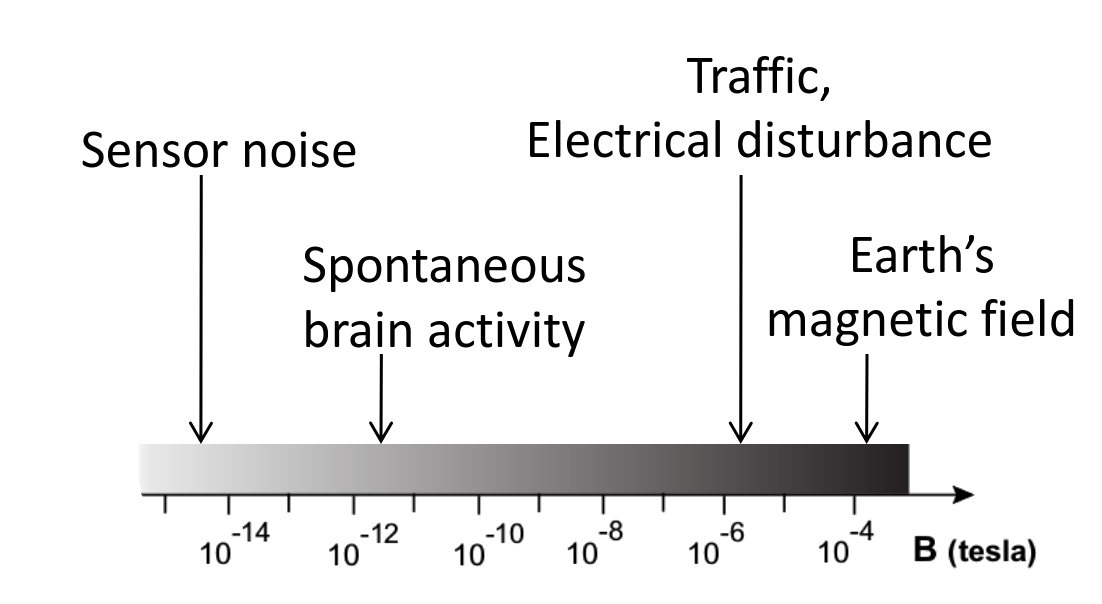
\includegraphics[height=8em]{scale_electro}
    \column{.5\textwidth}
    \vskip3em
    \hskip2em
    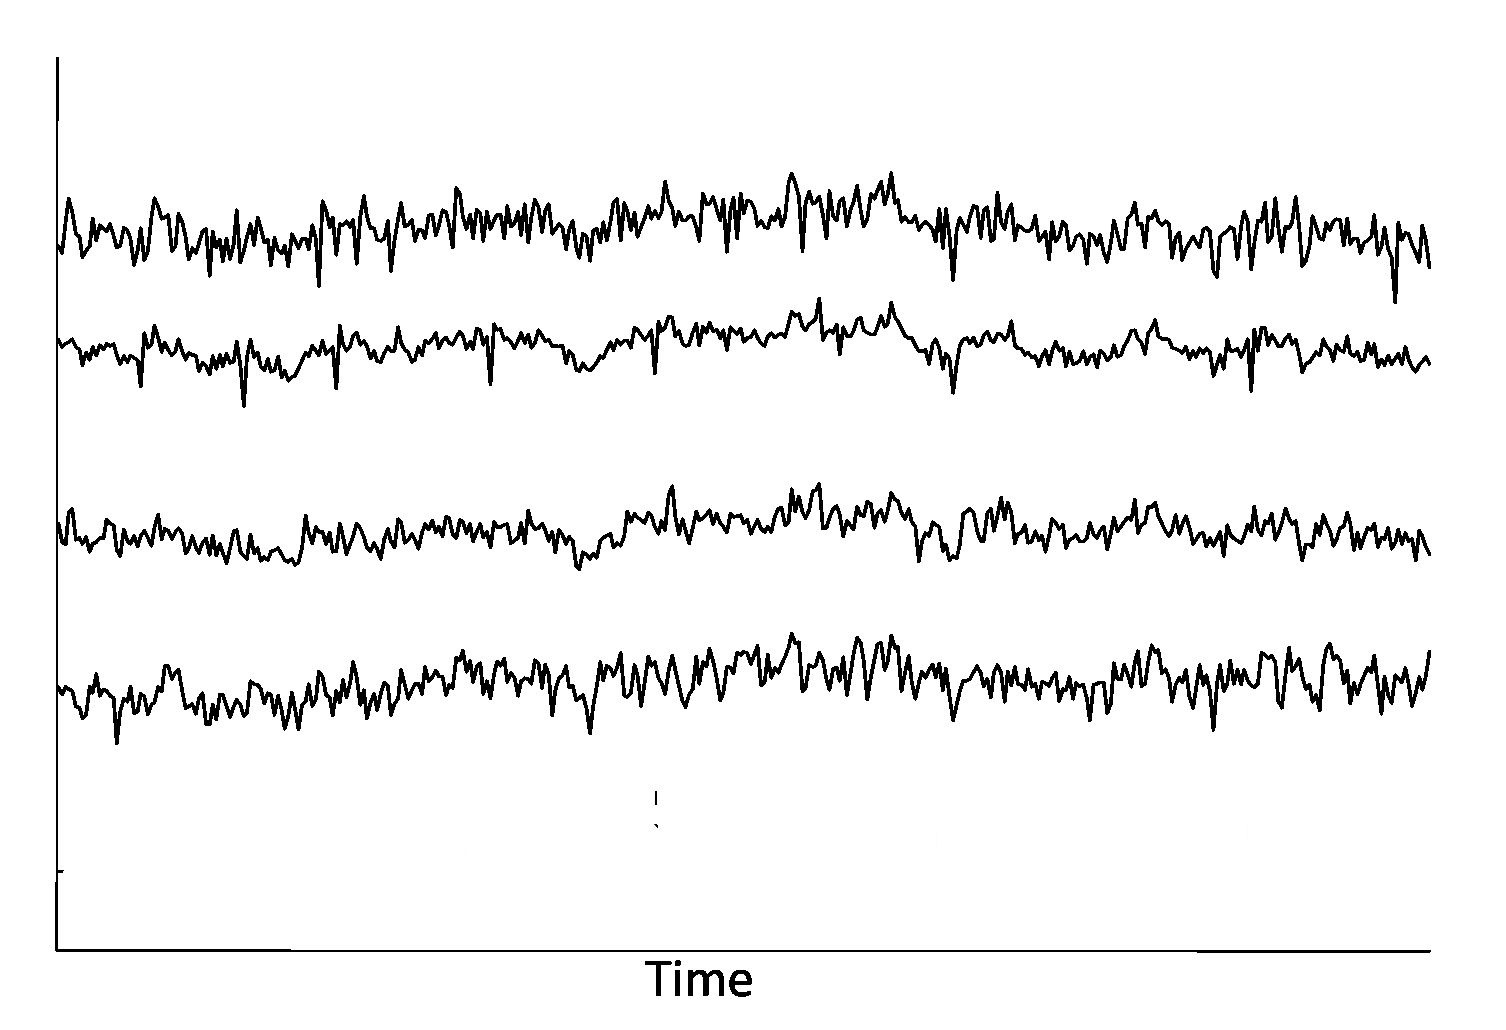
\includegraphics[height=8em]{multivariate_eeg}
\end{columns}
\end{frame}

\begin{frame}{Goal: Study Oscillation in Neural Data}

\textbf{}Oscillations are believed to play an important role in cognitive functions.\\[3em]
Many studies rely on Fourier or wavelet analyses:\\[.5em]
\begin{itemize}\itemsep1em
\item Easy interpretation,
\item Standard analysis \eg{} canonical bands alpha, beta or theta.\\\mycite{buzsaki2006rhythms}
\end{itemize}

\end{frame}

\begin{frame}{Goal: Study Oscillation in Neural Data}

However, some brain rhythms are not sinusoidal, \eg{} mu-waves.\\\mycite{hari2006action}\\
\hskip5em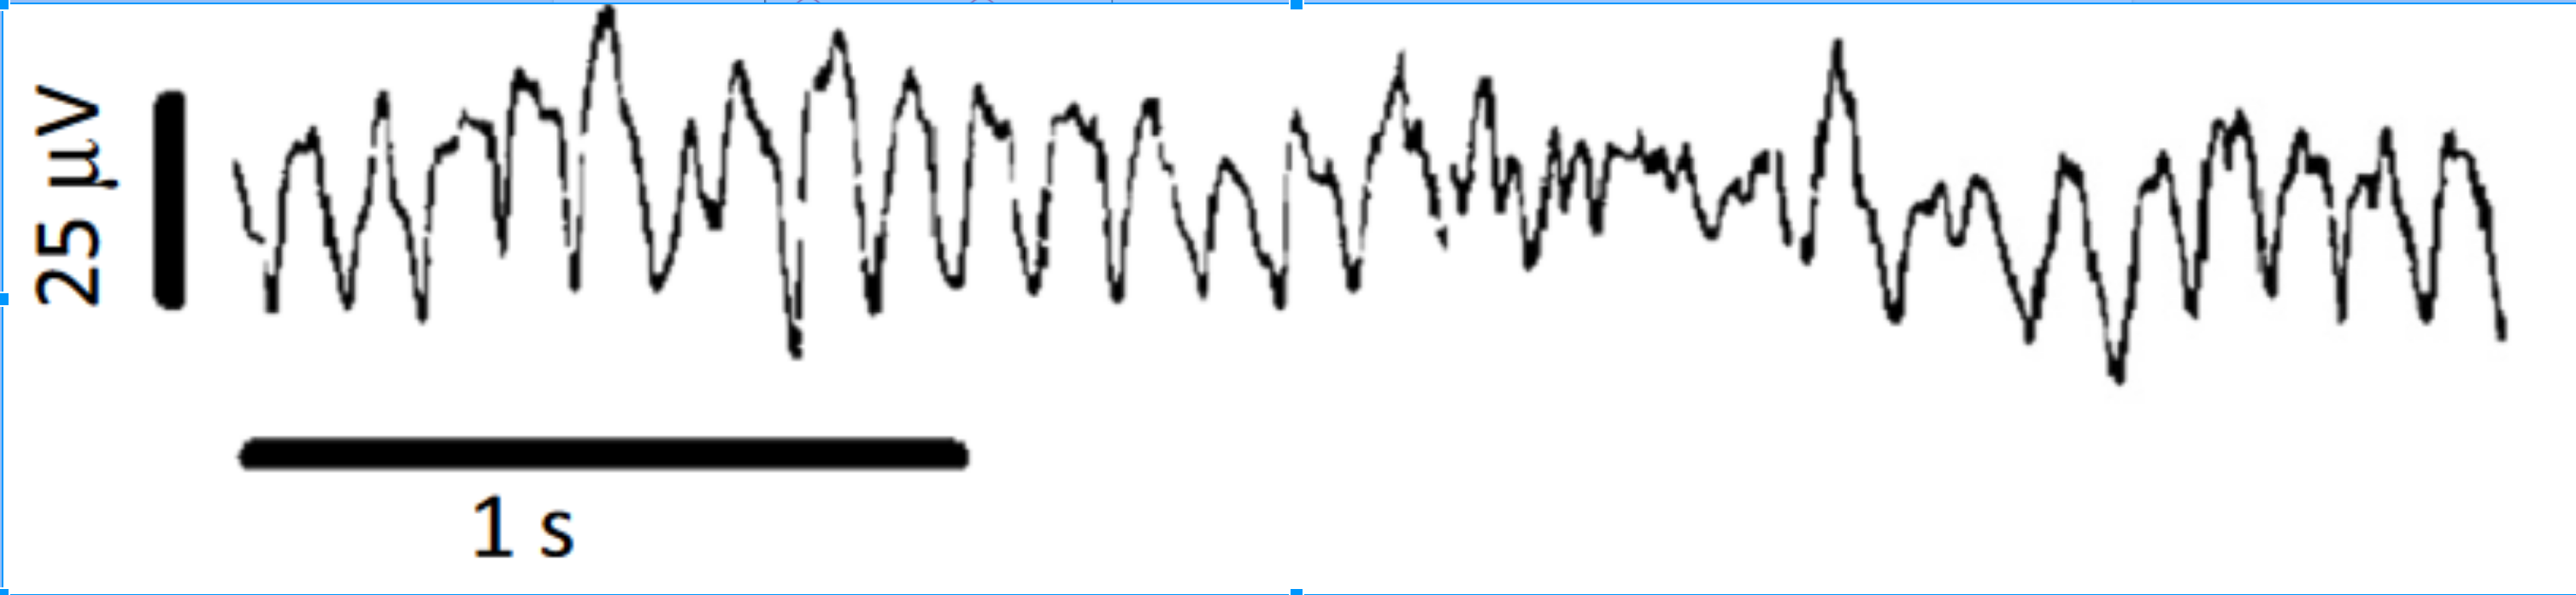
\includegraphics[width=.7\textwidth]{waveform}\\
and filtering degrades waveforms\\
\hskip8em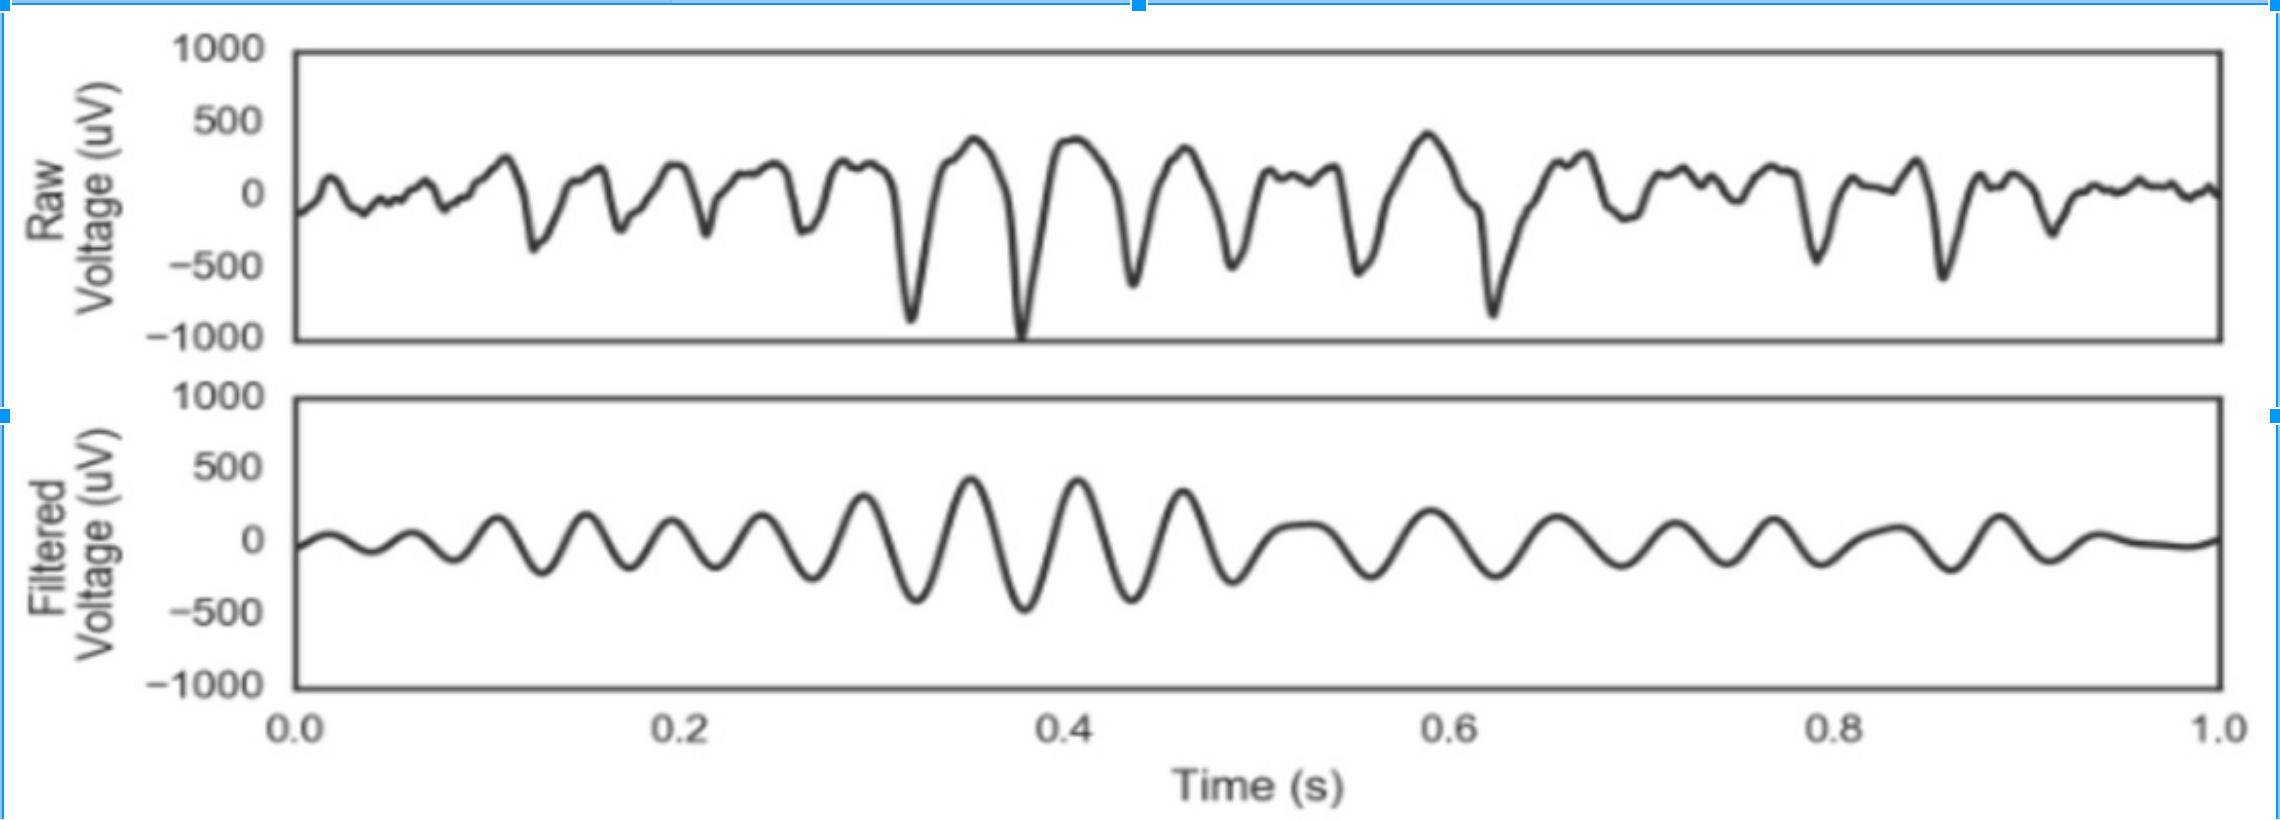
\includegraphics[width=.5\textwidth]{filtering_brain}


\strongpoint{Can we do better with data-driven approach?}
\end{frame}


\begin{frame}{Pattern recovery}
Evolution of the recovery loss with $\sigma$ for different values of $P$. Using more channels improves the recovery of the original patterns.\\[1em]
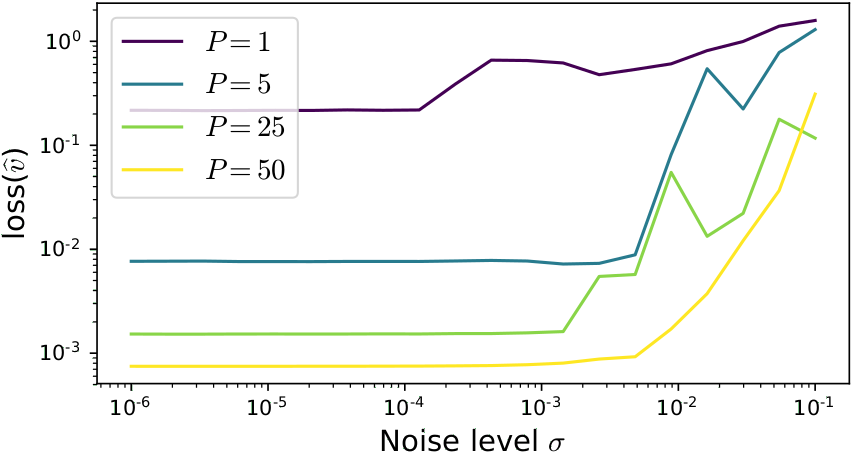
\includegraphics[width=\textwidth]{1D_vs_multi.png}
\end{frame}

\end{document}
